\subsection{Rate-limited, repetition 1}
\begin{figure}[H]\centering
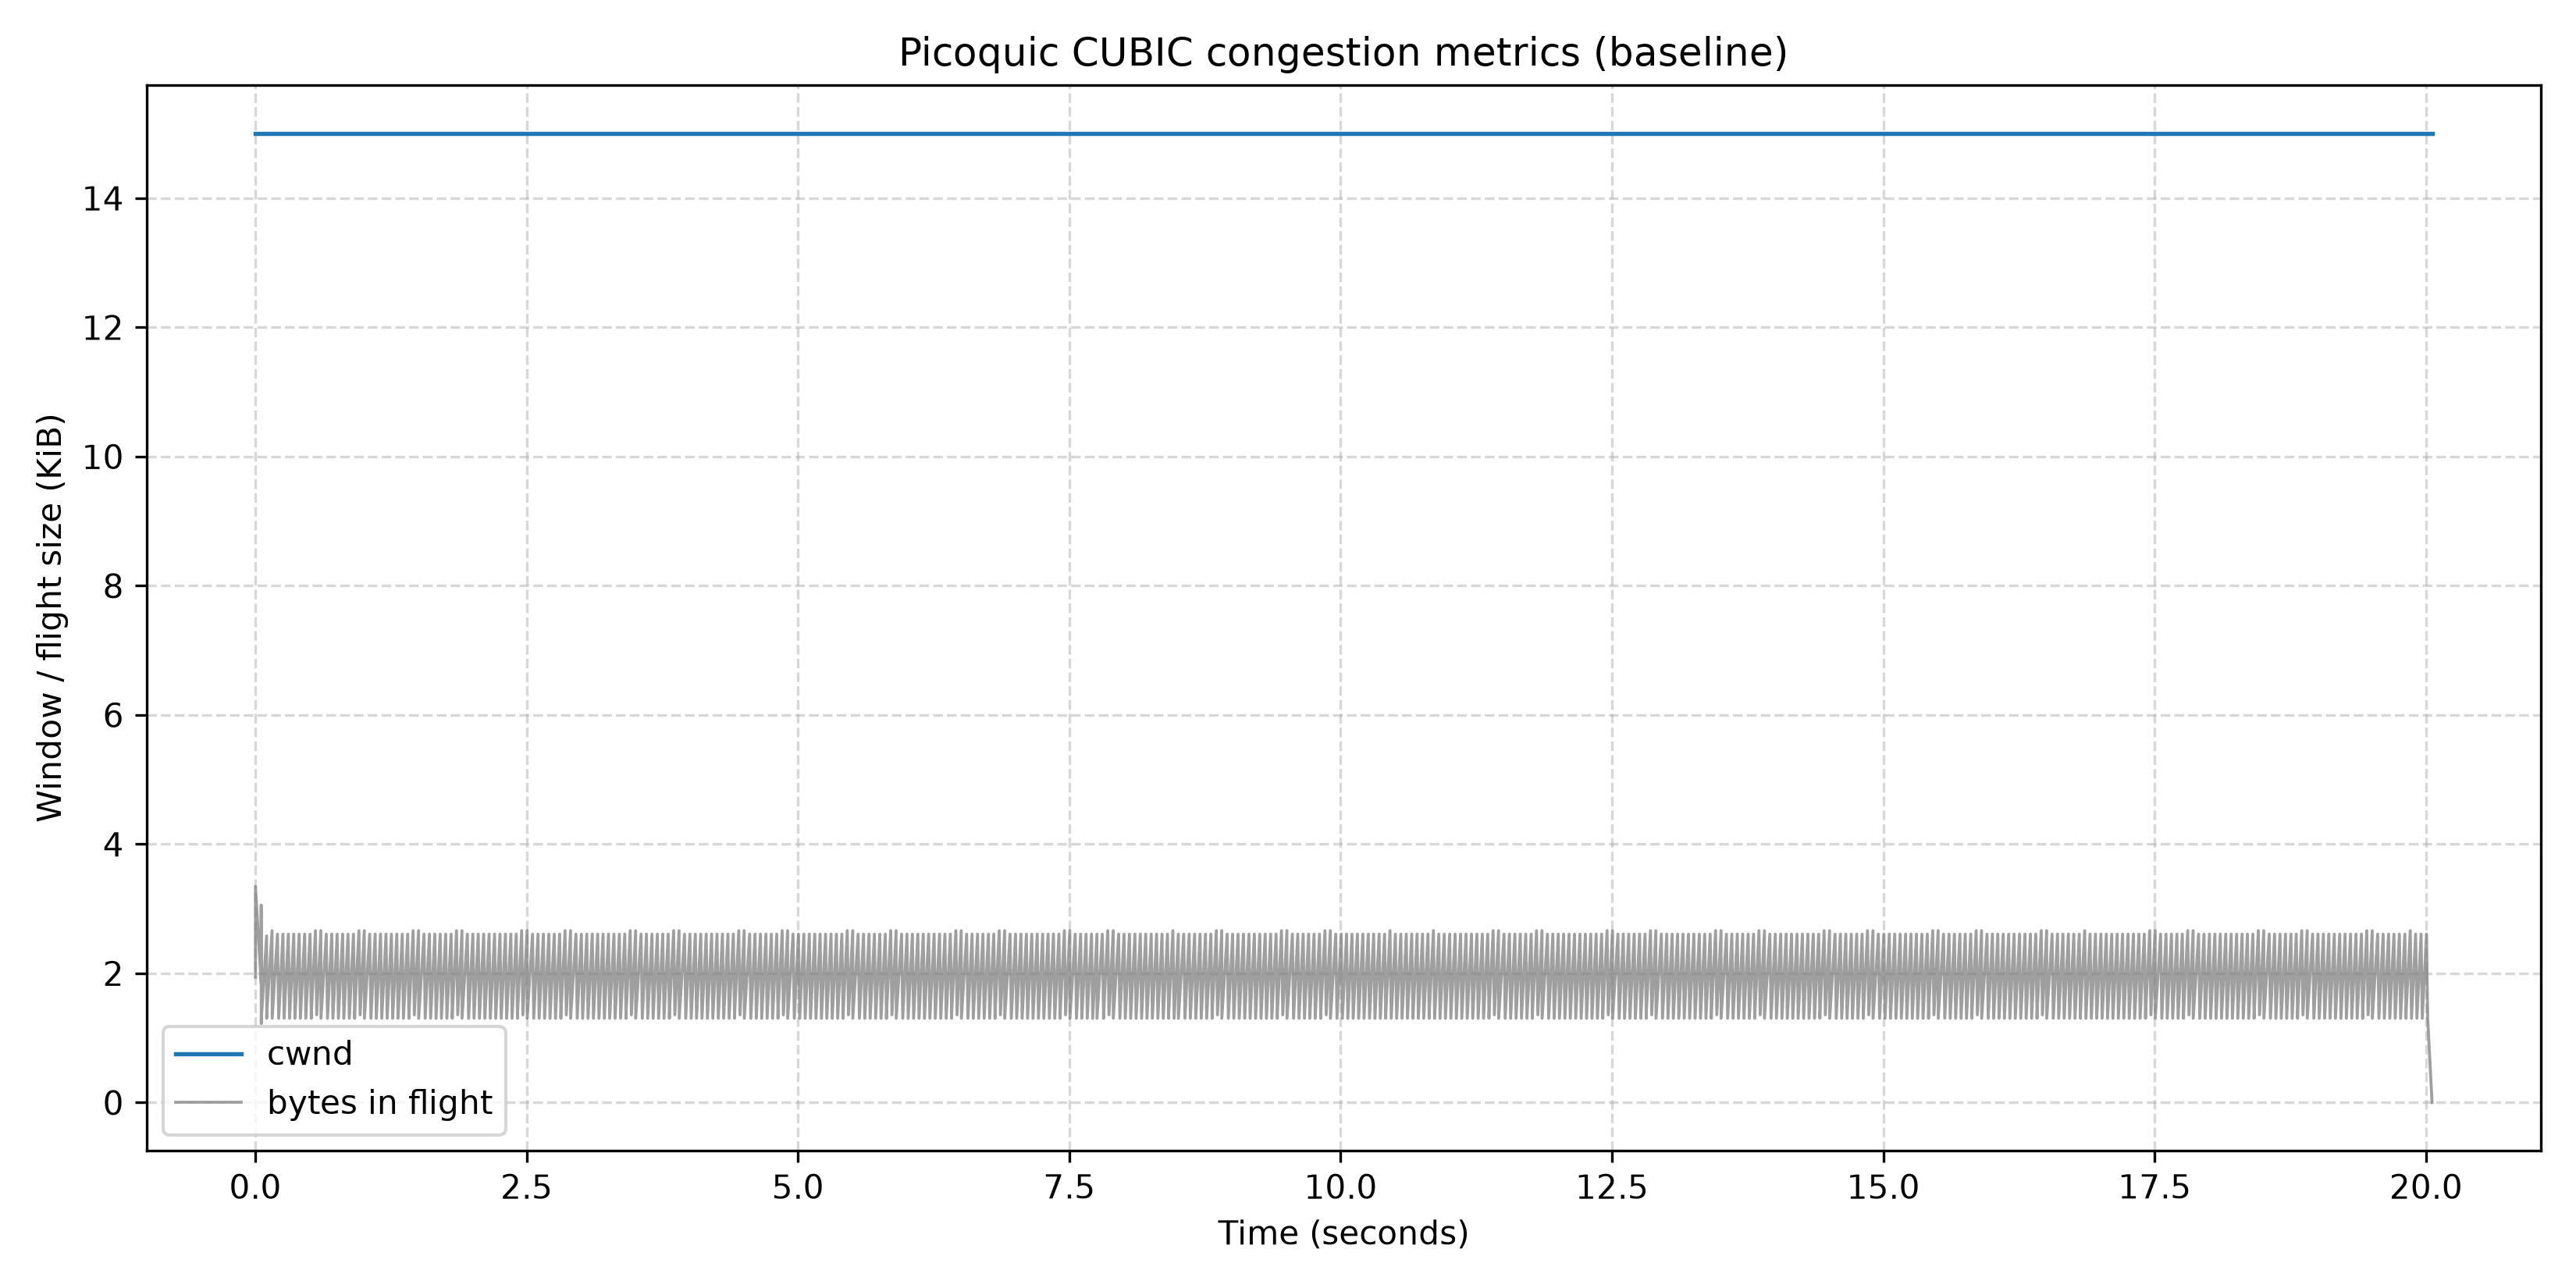
\includegraphics[width=0.92\textwidth]{plots/rate-limited-baseline-1.png}
\caption{Baseline: final cwnd 15.00 KiB; time-weighted mean 15.00 KiB; throughput 0.190 Mbit/s.}\end{figure}
\begin{figure}[H]\centering
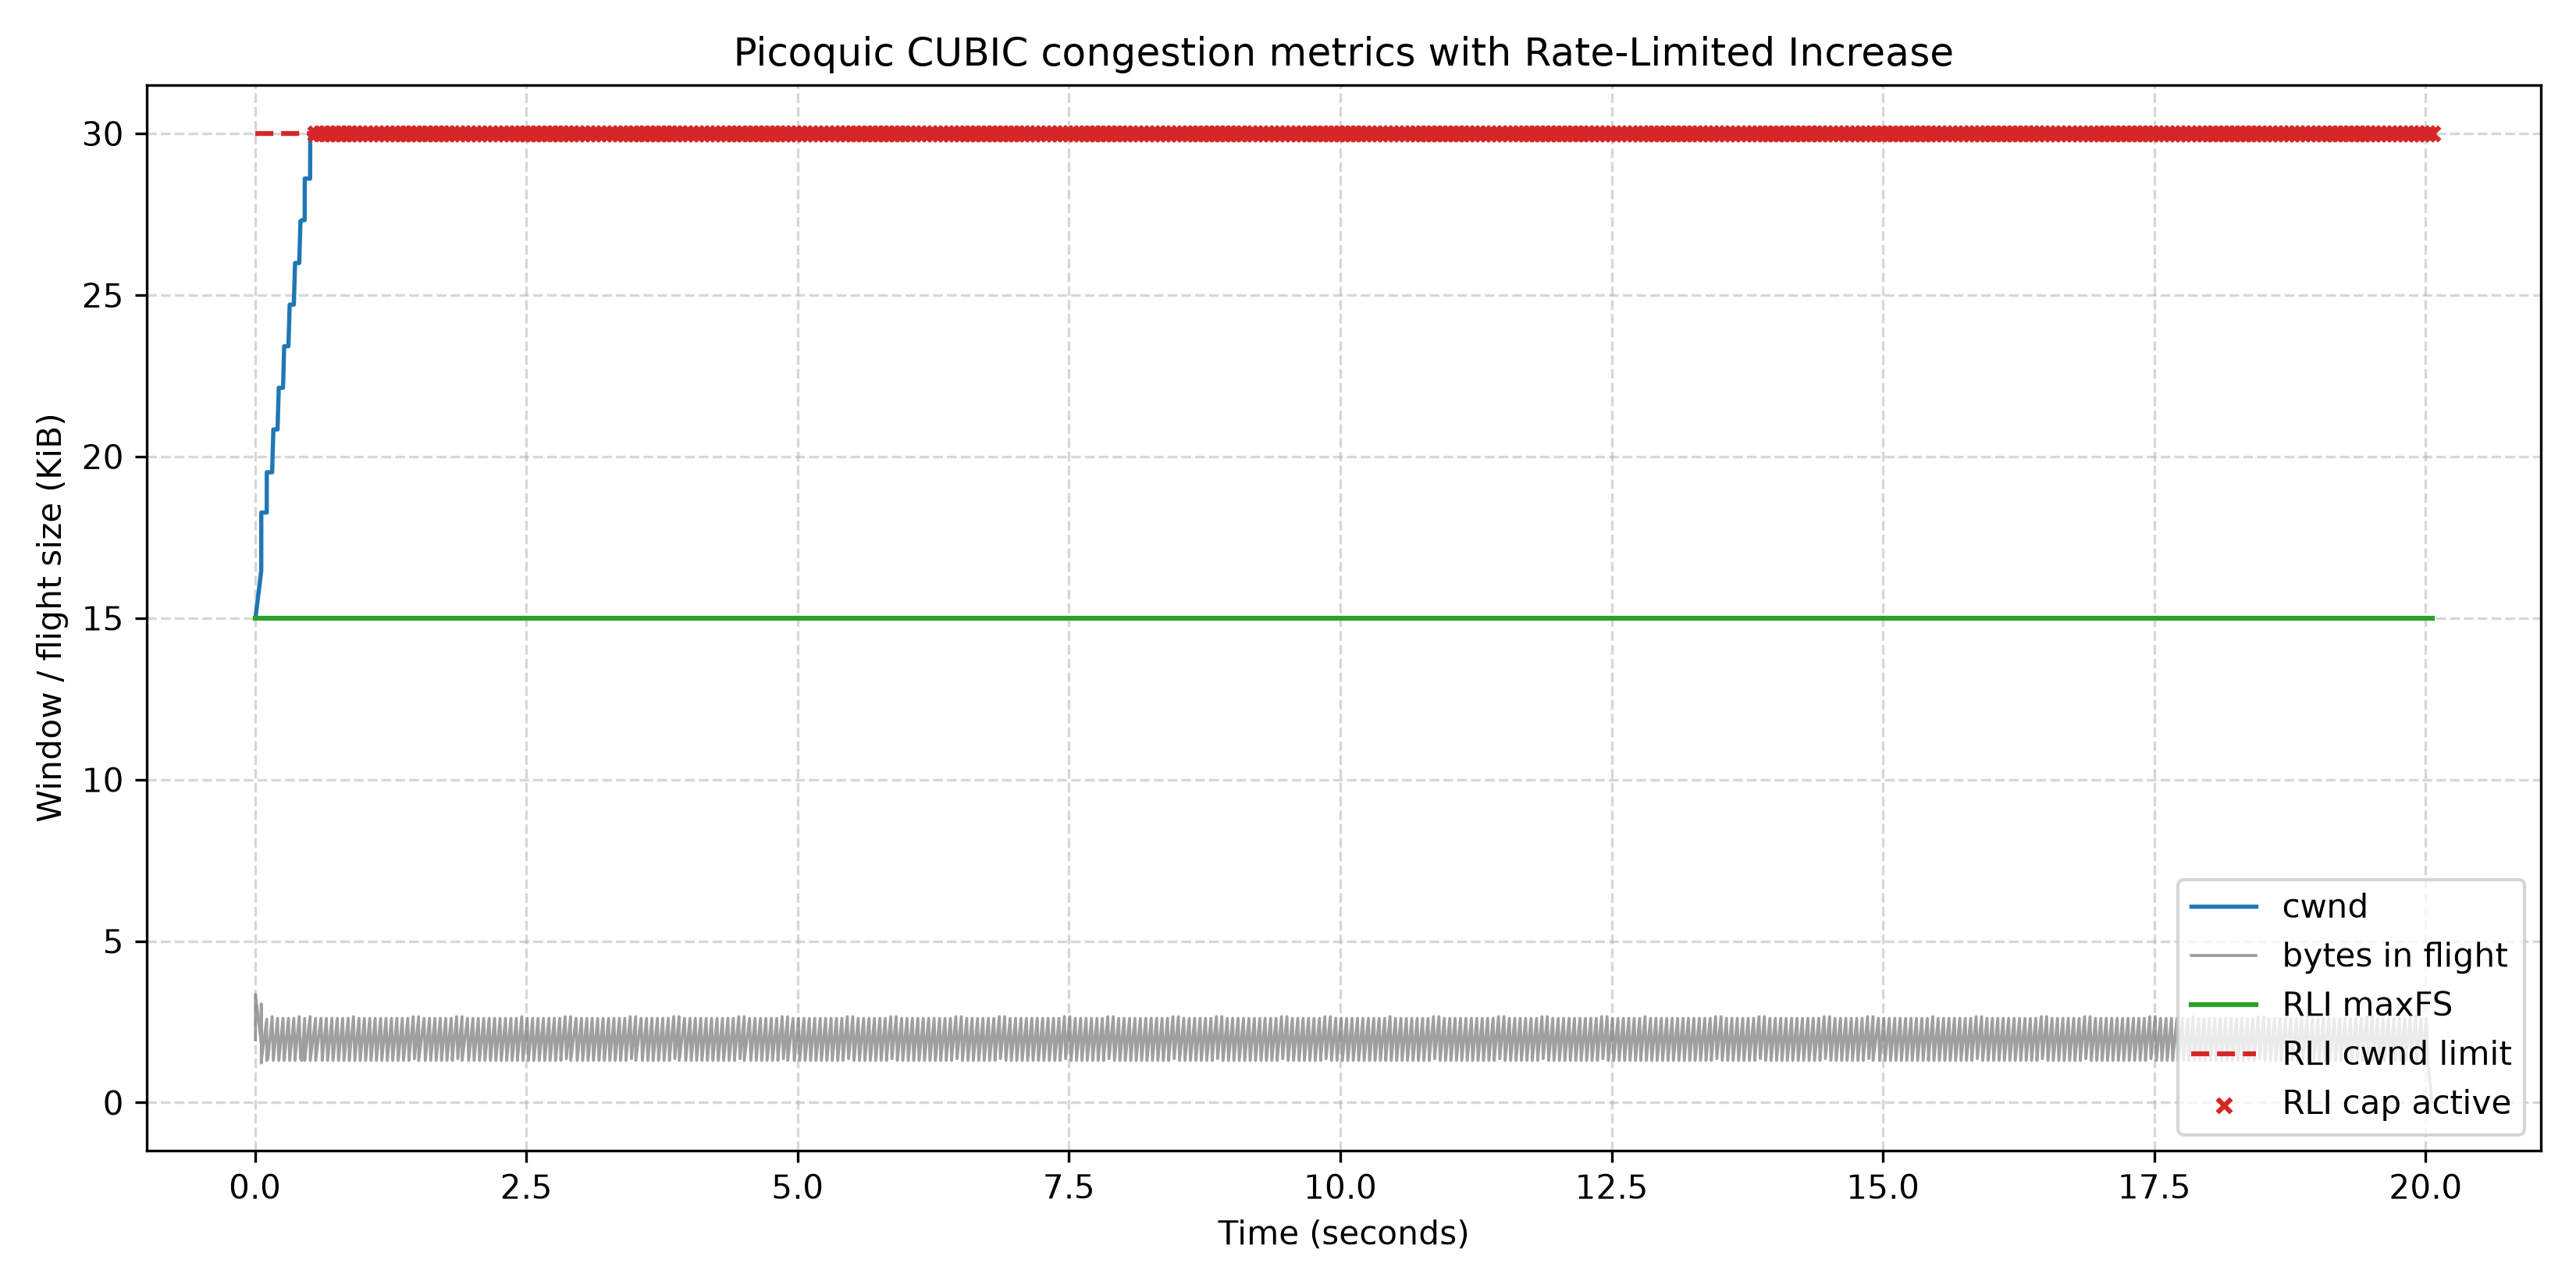
\includegraphics[width=0.92\textwidth]{plots/rate-limited-rli-1.png}
\caption{Rli: final cwnd 30.00 KiB; time-weighted mean 29.81 KiB; throughput 0.190 Mbit/s.}\end{figure}
These matched traces isolate rate-limited window growth. RLI permits bounded ACK-driven growth; application supply still controls throughput.
\clearpage\subsection{Rate-limited, repetition 2}
\begin{figure}[H]\centering
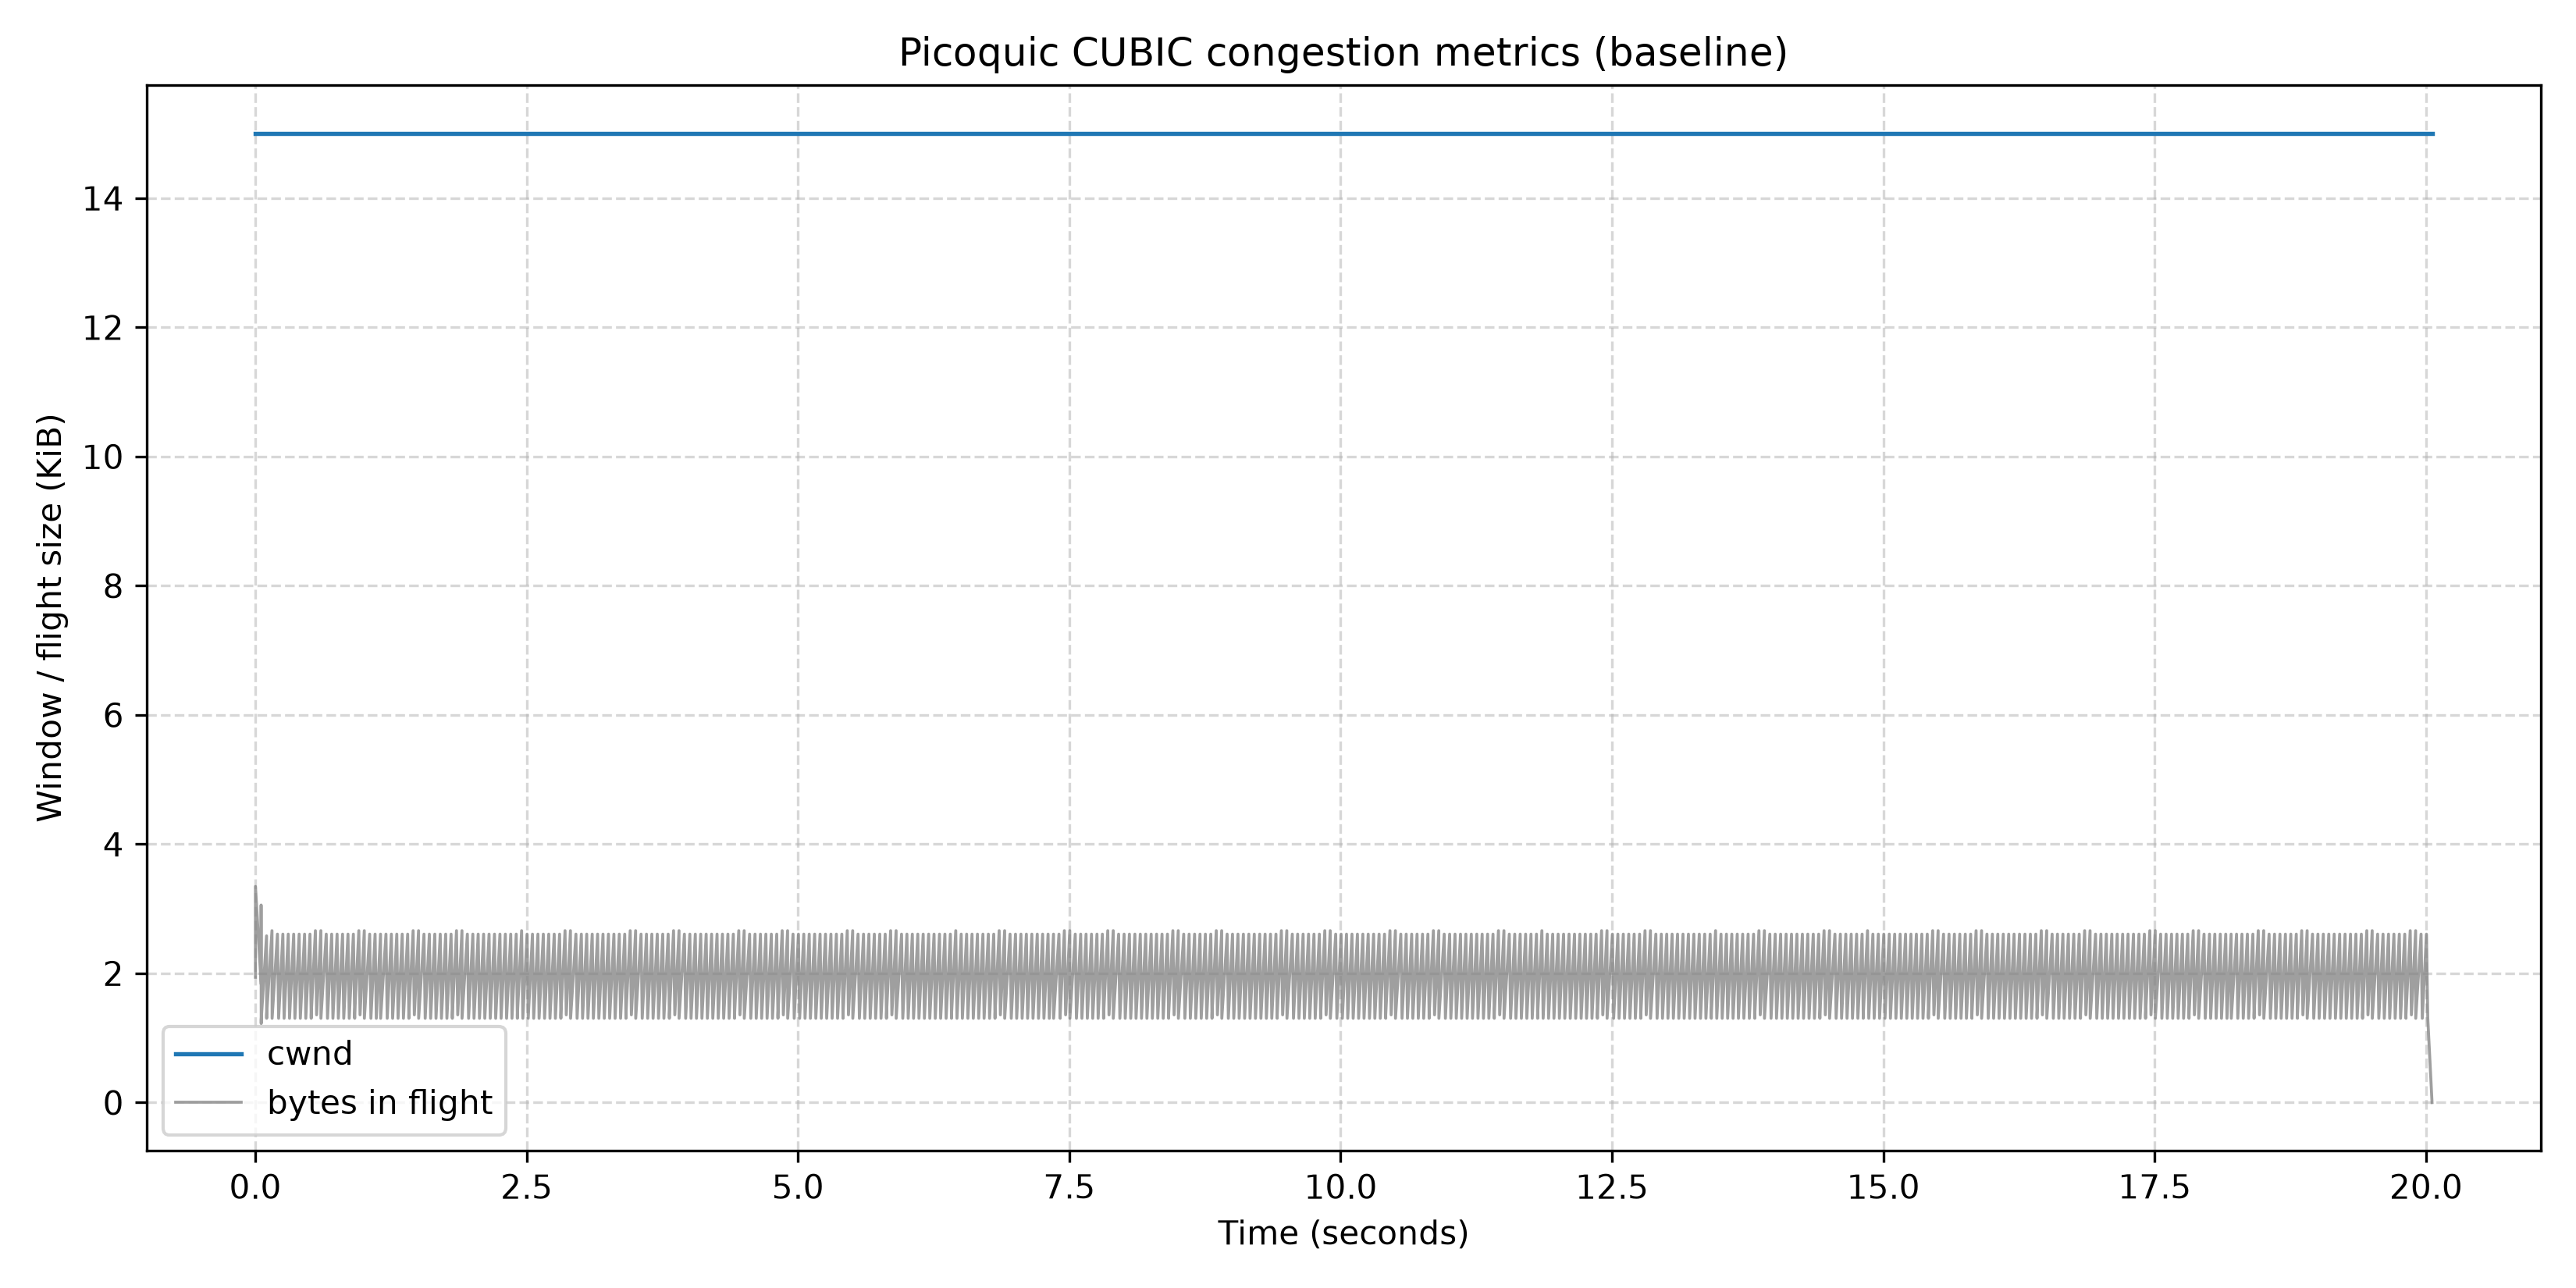
\includegraphics[width=0.92\textwidth]{plots/rate-limited-baseline-2.png}
\caption{Baseline: final cwnd 15.00 KiB; time-weighted mean 15.00 KiB; throughput 0.190 Mbit/s.}\end{figure}
\begin{figure}[H]\centering
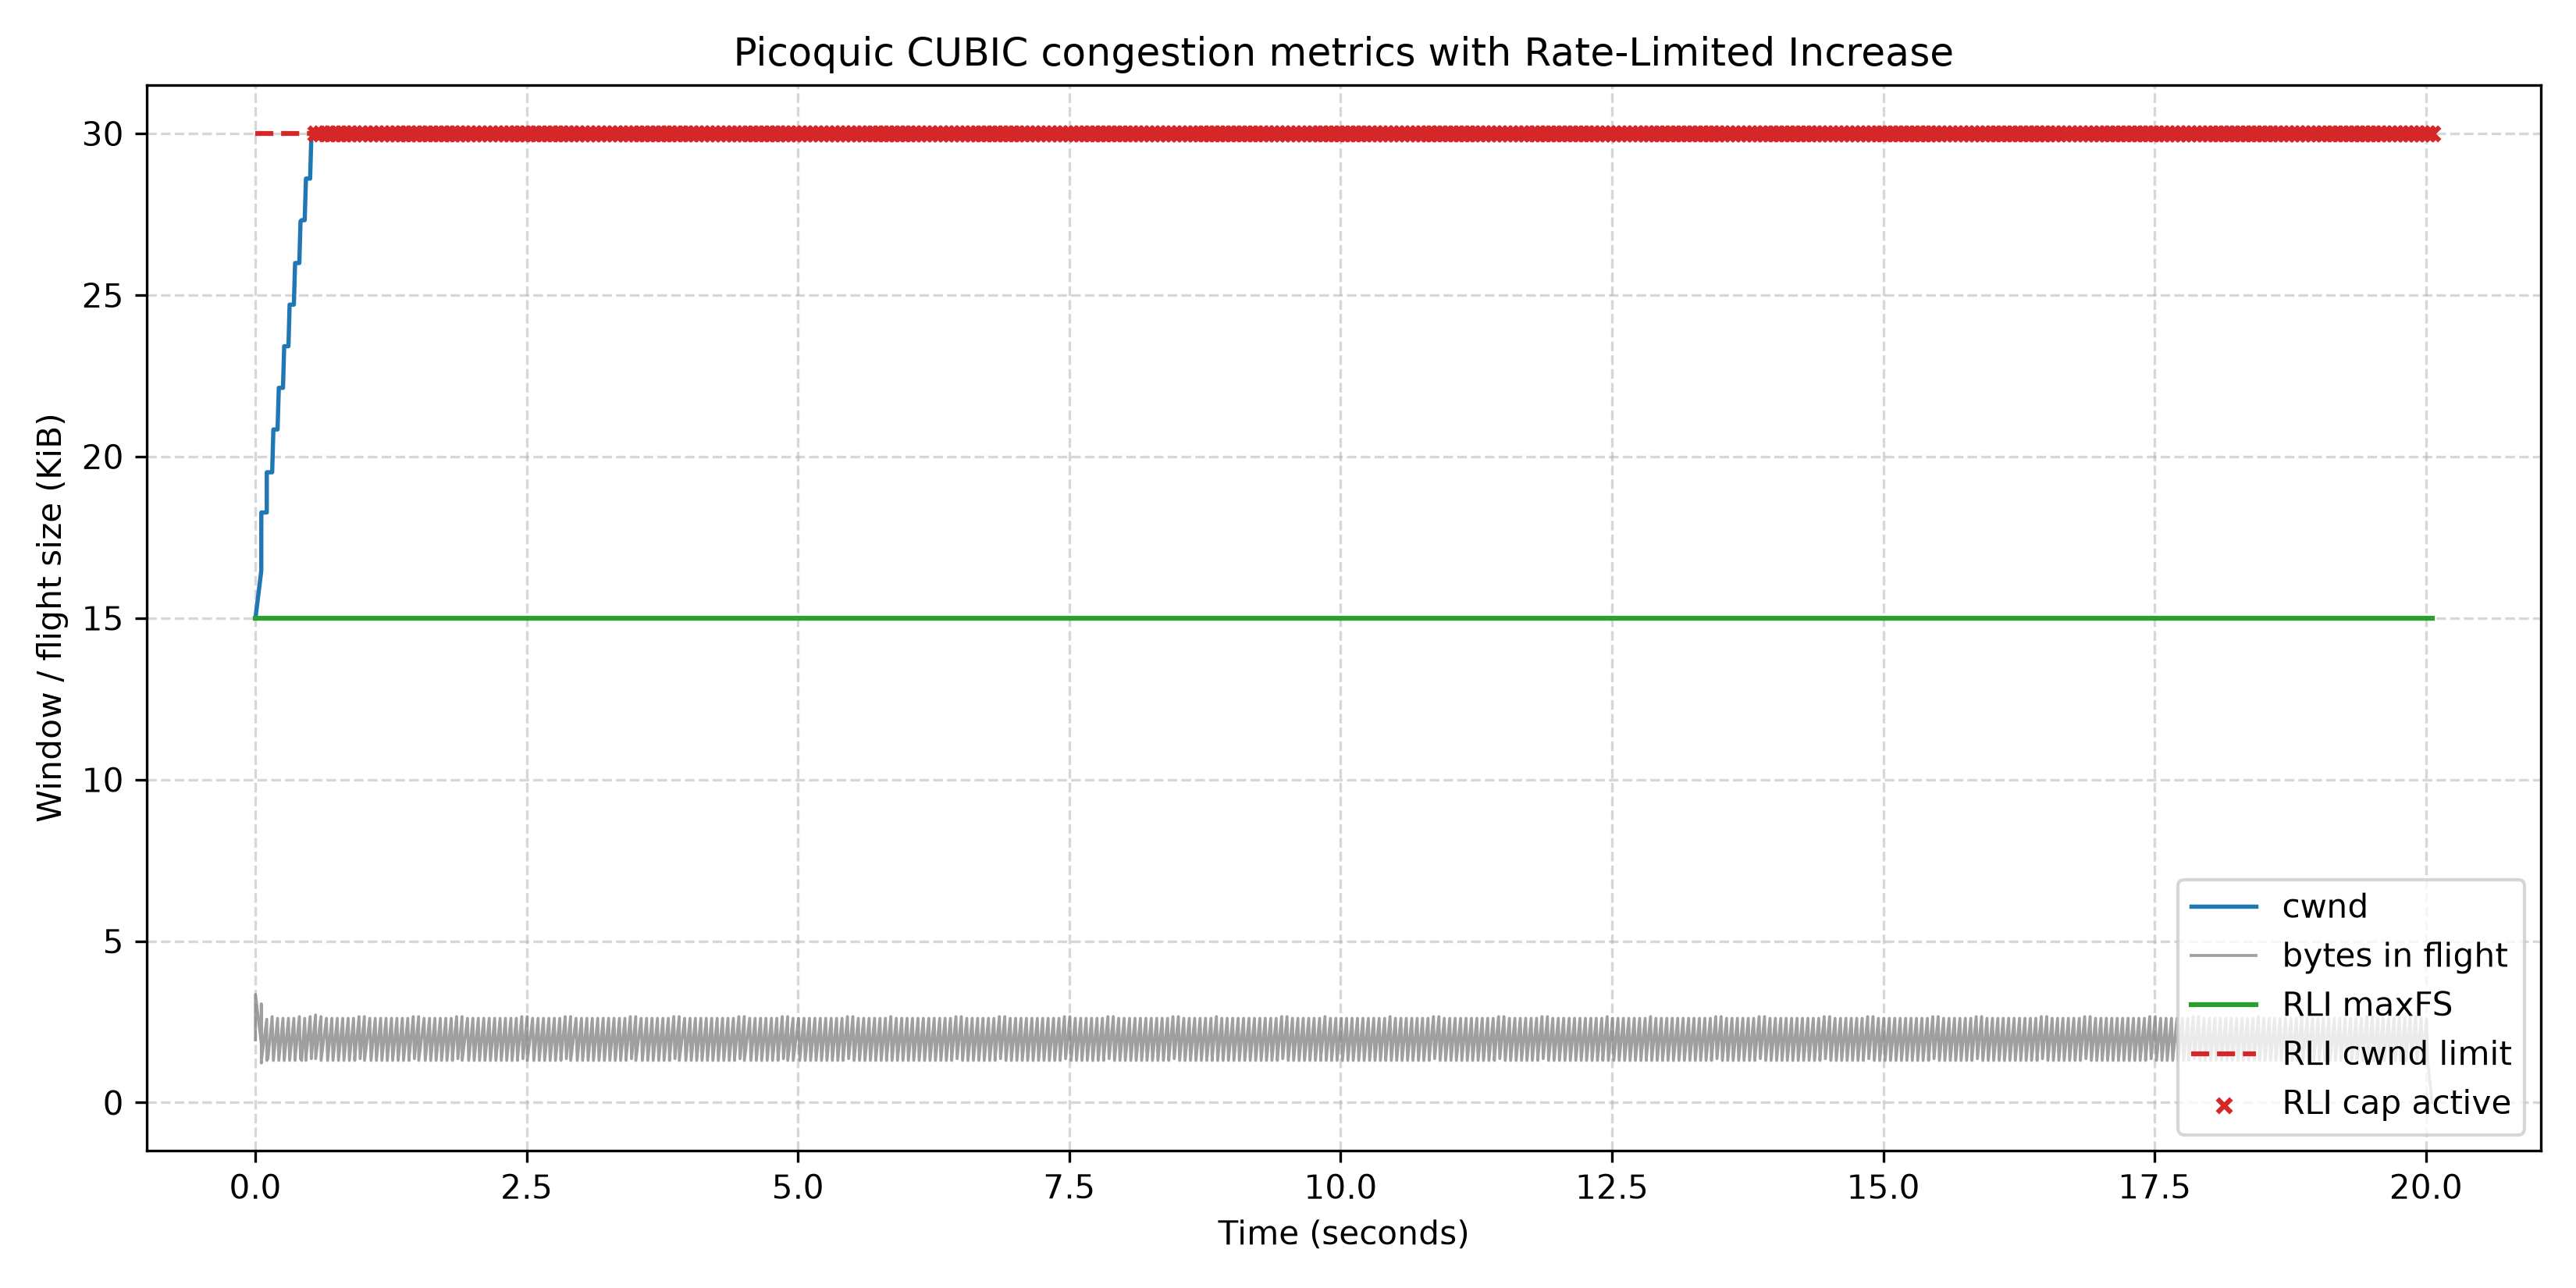
\includegraphics[width=0.92\textwidth]{plots/rate-limited-rli-2.png}
\caption{Rli: final cwnd 30.00 KiB; time-weighted mean 29.81 KiB; throughput 0.190 Mbit/s.}\end{figure}
These matched traces isolate rate-limited window growth. RLI permits bounded ACK-driven growth; application supply still controls throughput.
\clearpage\subsection{Rate-limited, repetition 3}
\begin{figure}[H]\centering
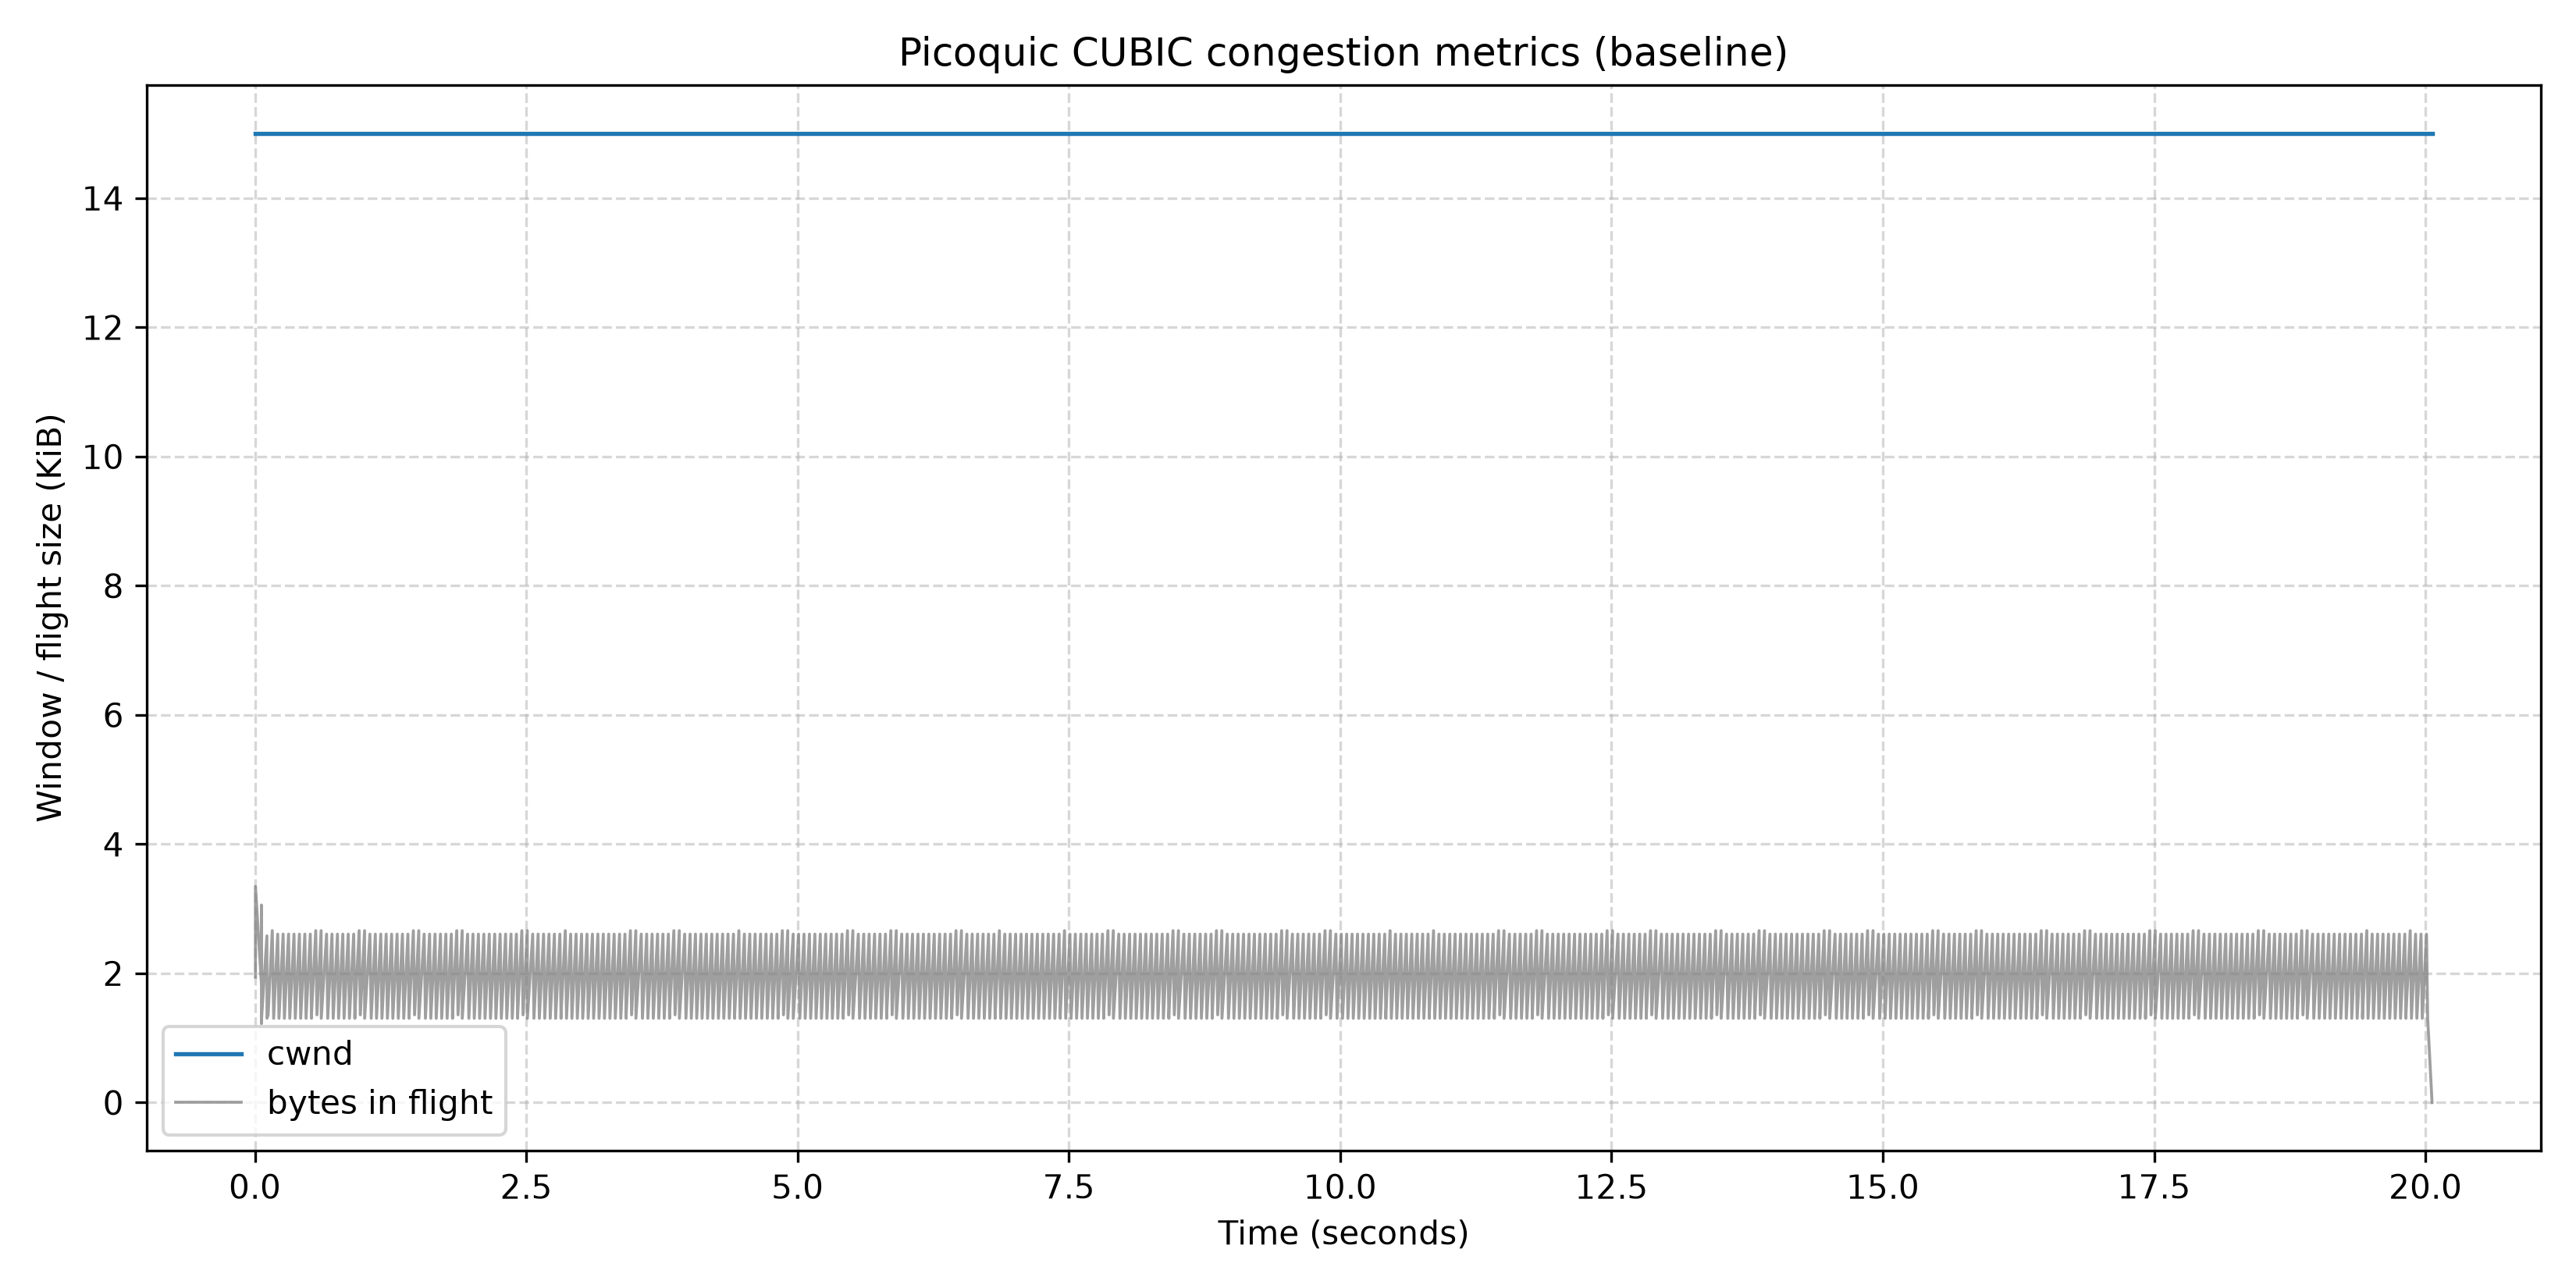
\includegraphics[width=0.92\textwidth]{plots/rate-limited-baseline-3.png}
\caption{Baseline: final cwnd 15.00 KiB; time-weighted mean 15.00 KiB; throughput 0.190 Mbit/s.}\end{figure}
\begin{figure}[H]\centering
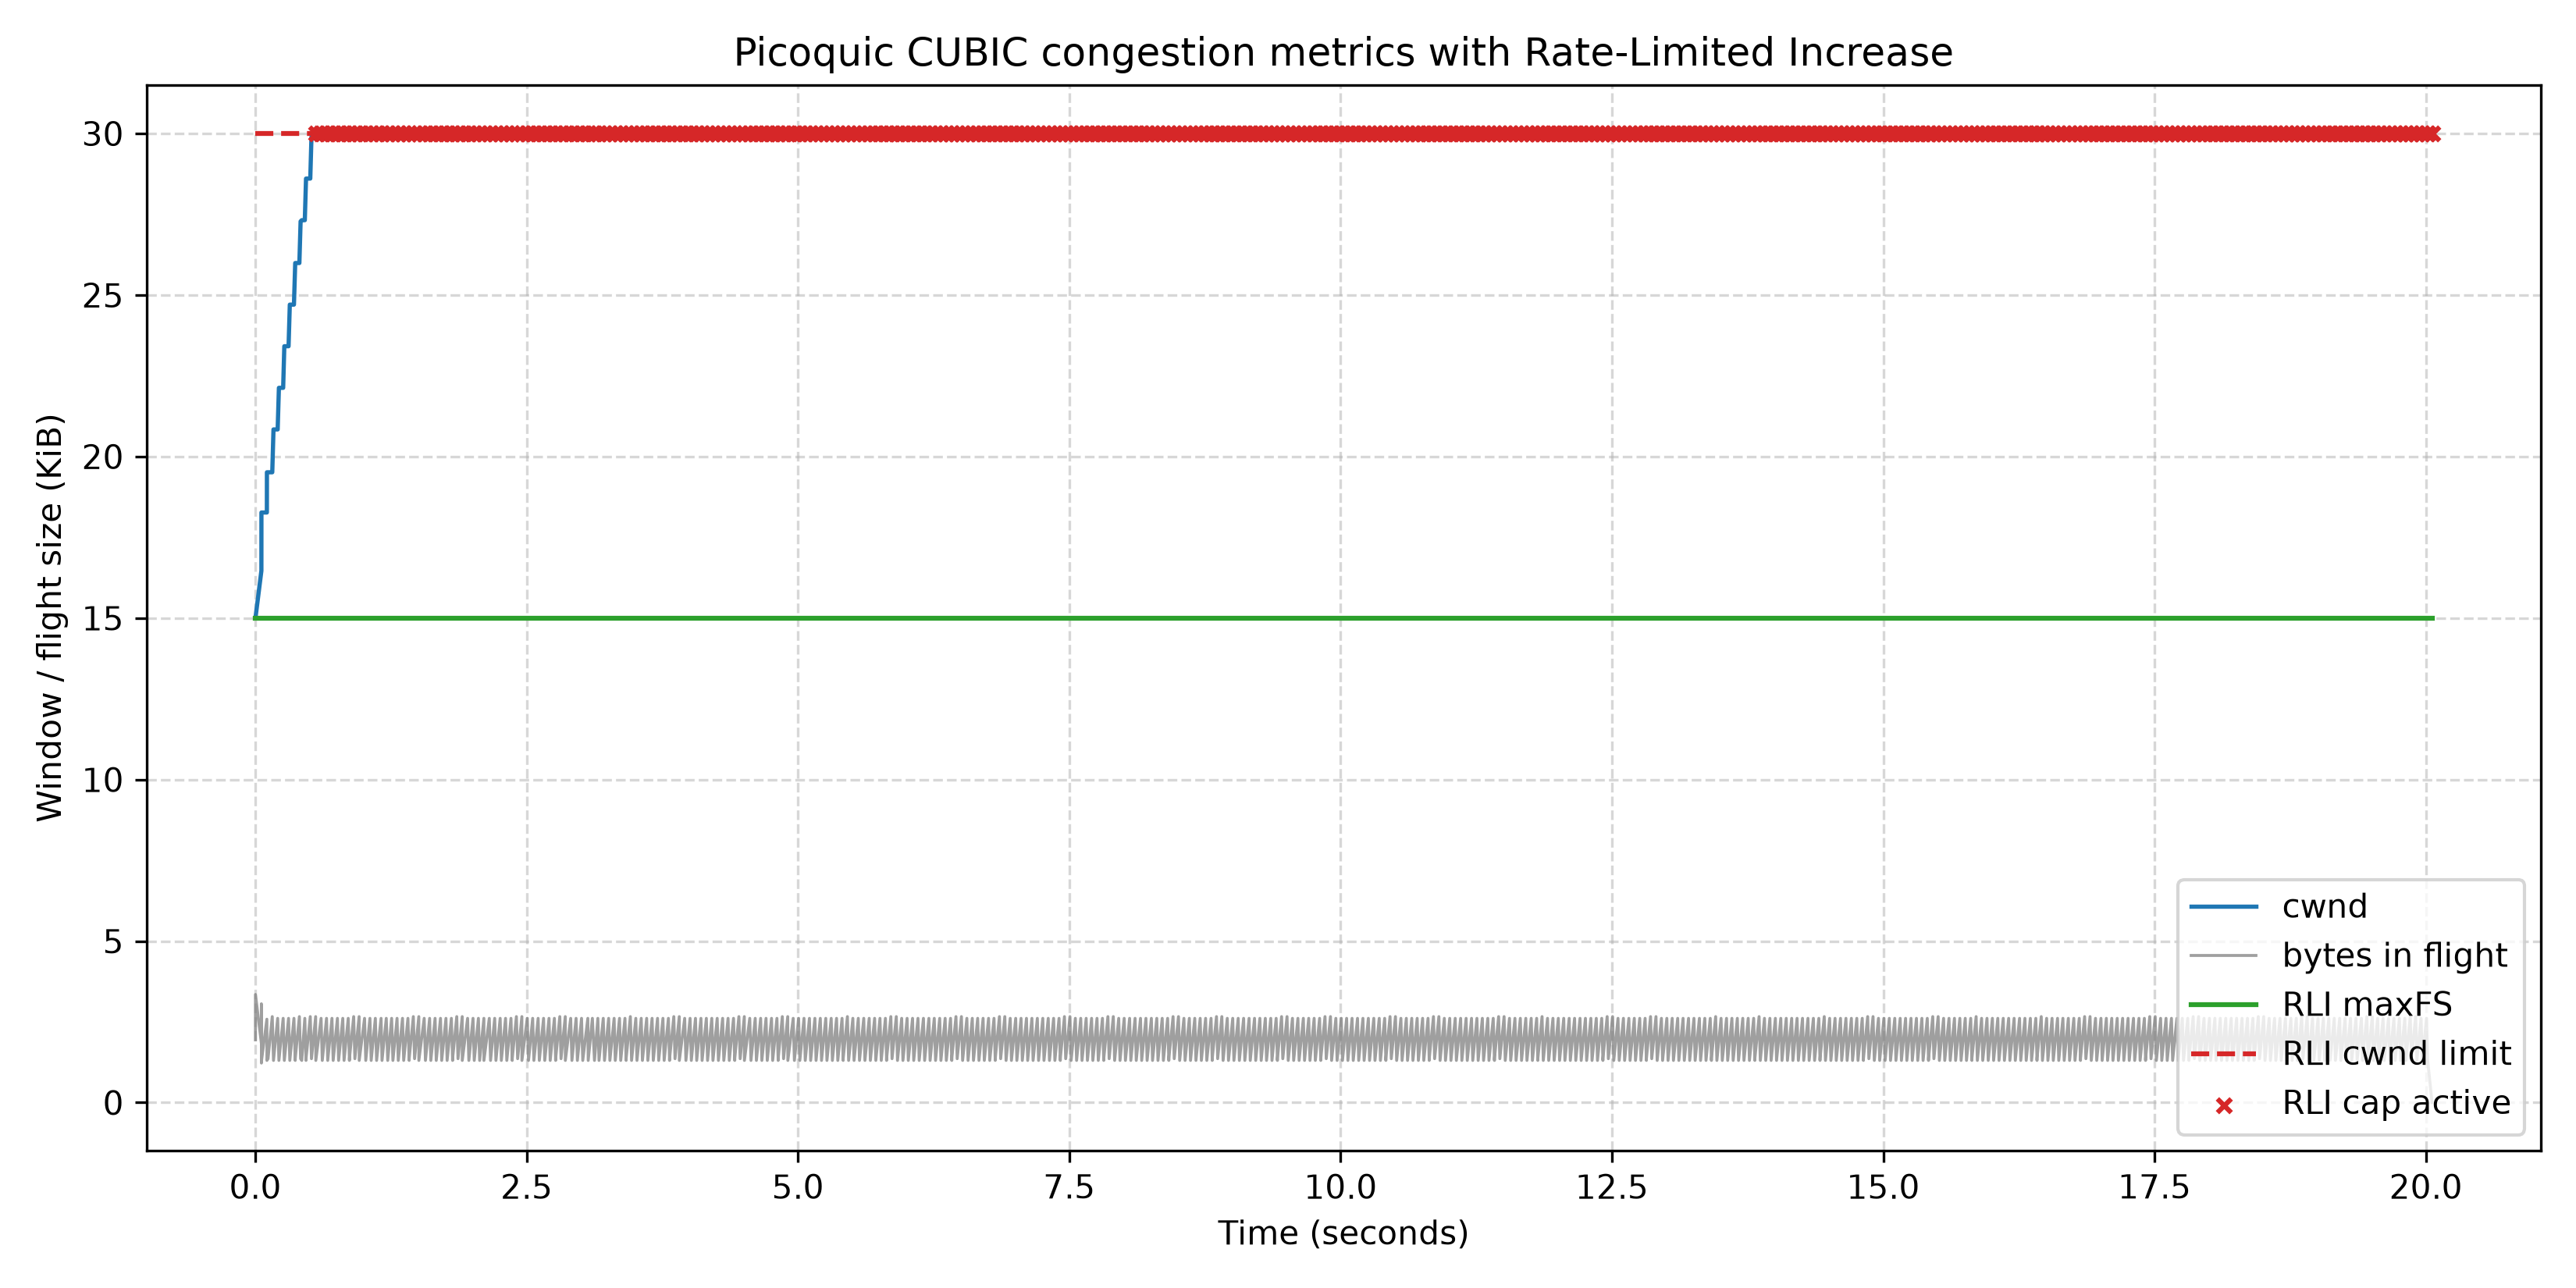
\includegraphics[width=0.92\textwidth]{plots/rate-limited-rli-3.png}
\caption{Rli: final cwnd 30.00 KiB; time-weighted mean 29.81 KiB; throughput 0.190 Mbit/s.}\end{figure}
These matched traces isolate rate-limited window growth. RLI permits bounded ACK-driven growth; application supply still controls throughput.
\clearpage\subsection{Bulk control, repetition 1}
\begin{figure}[H]\centering
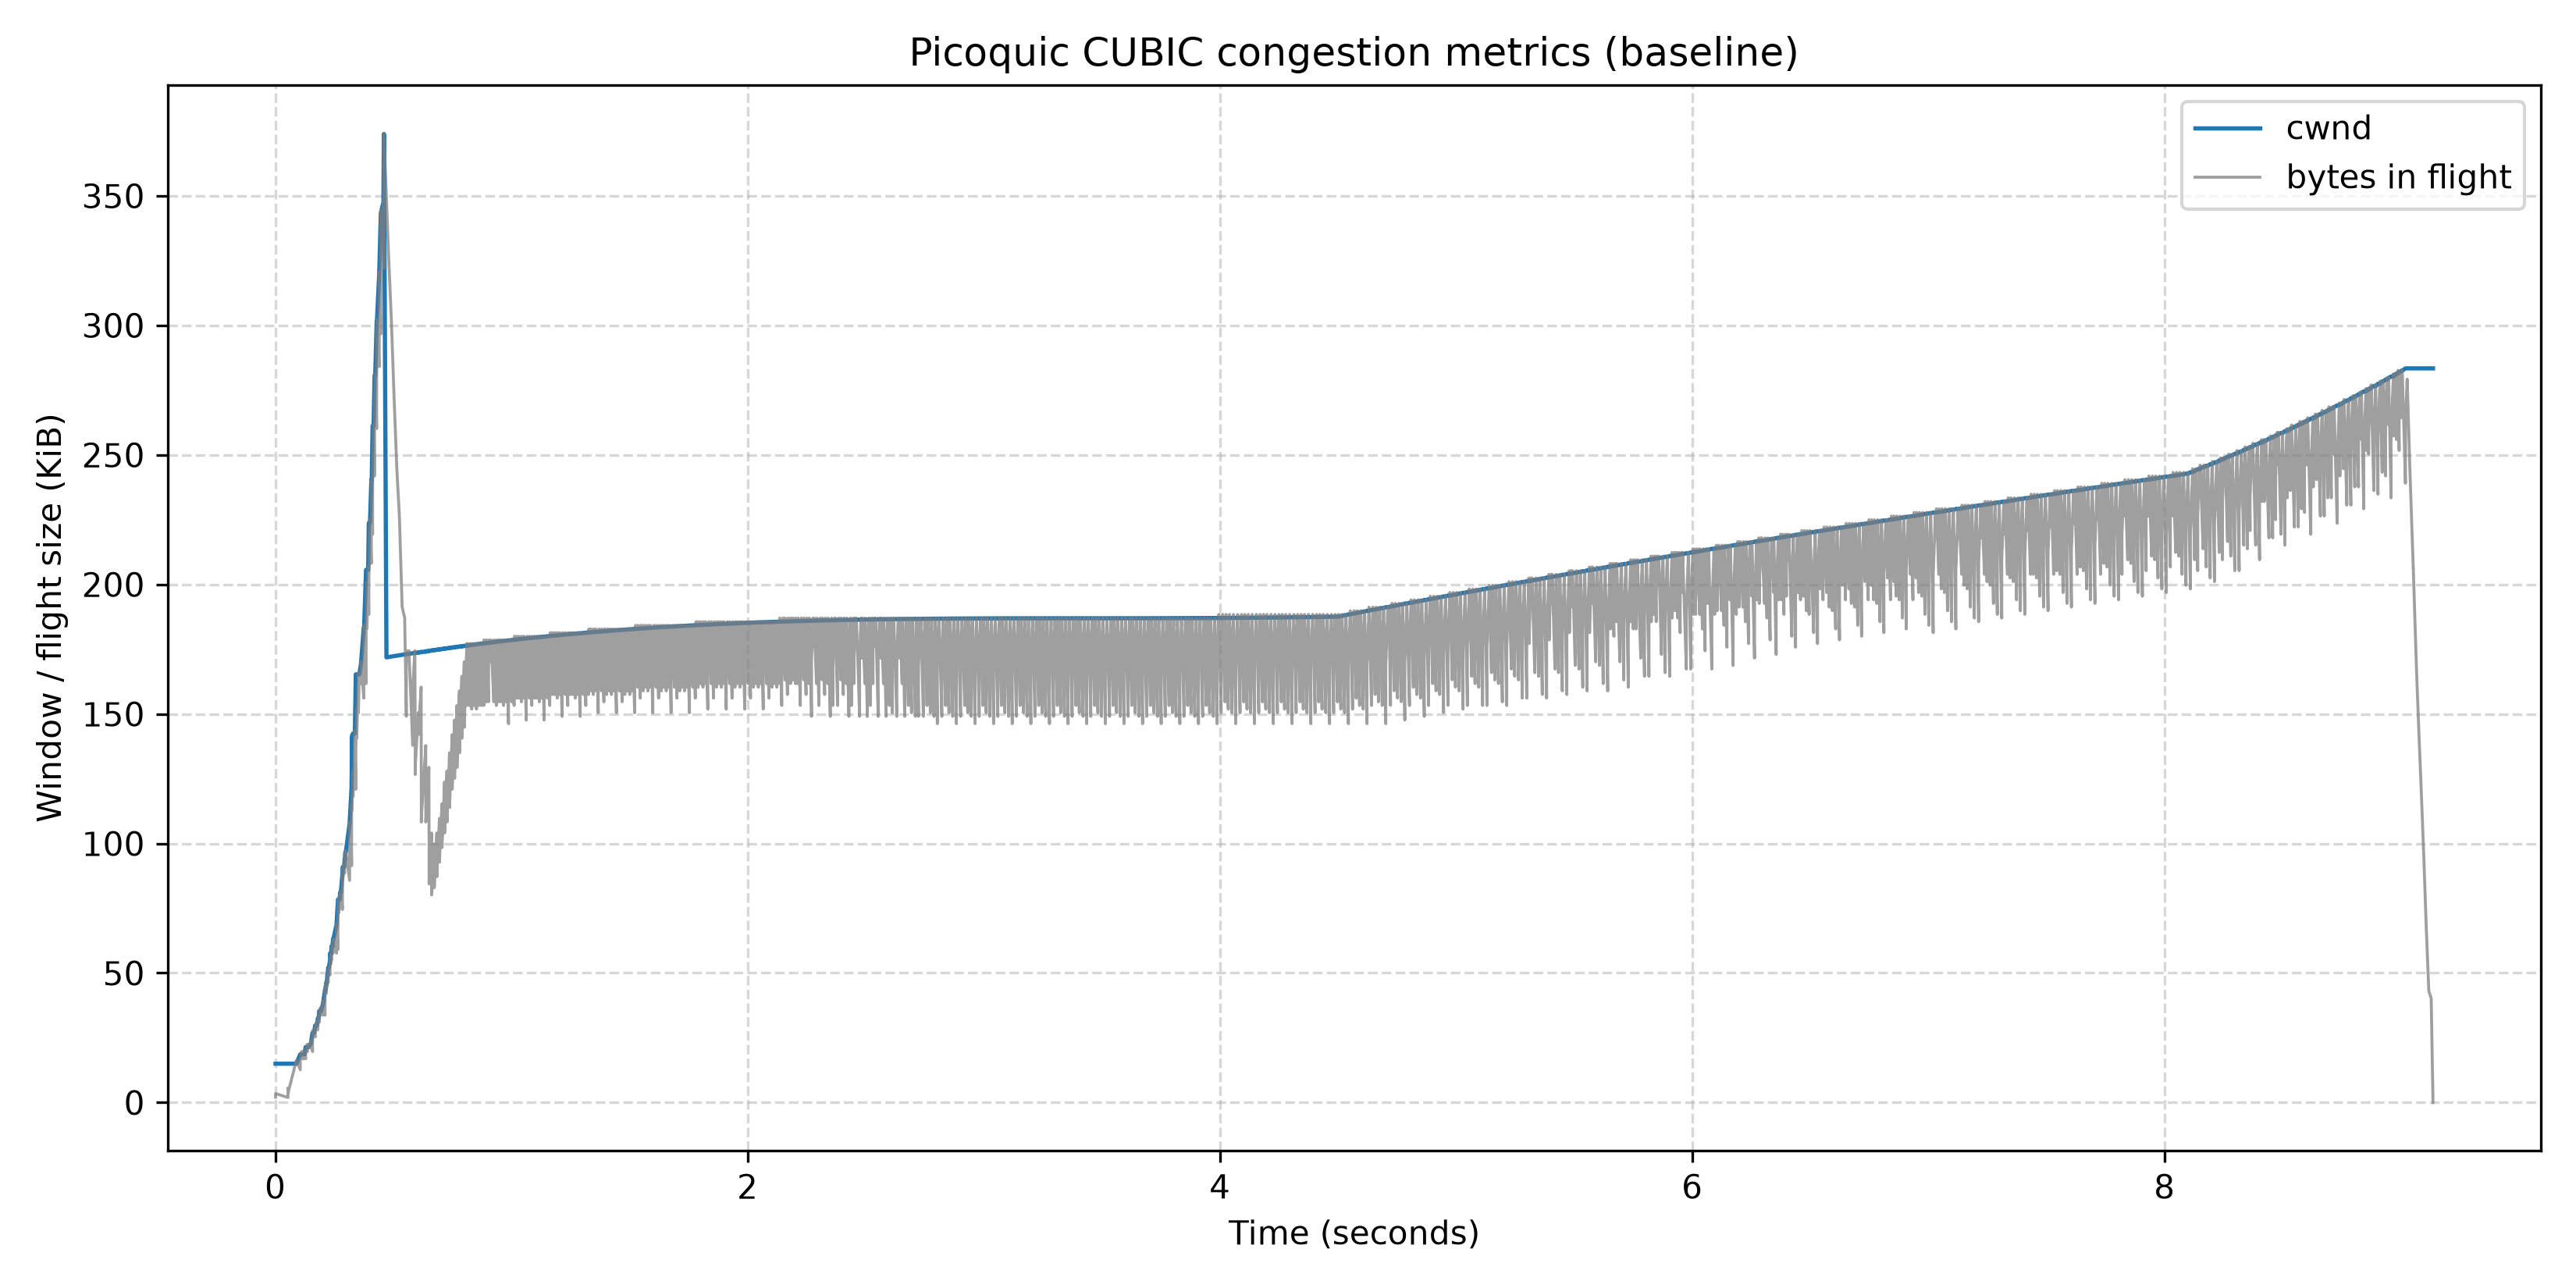
\includegraphics[width=0.92\textwidth]{plots/bulk-baseline-1.png}
\caption{Baseline: final cwnd 283.41 KiB; time-weighted mean 201.63 KiB; throughput 17.731 Mbit/s.}\end{figure}
\begin{figure}[H]\centering
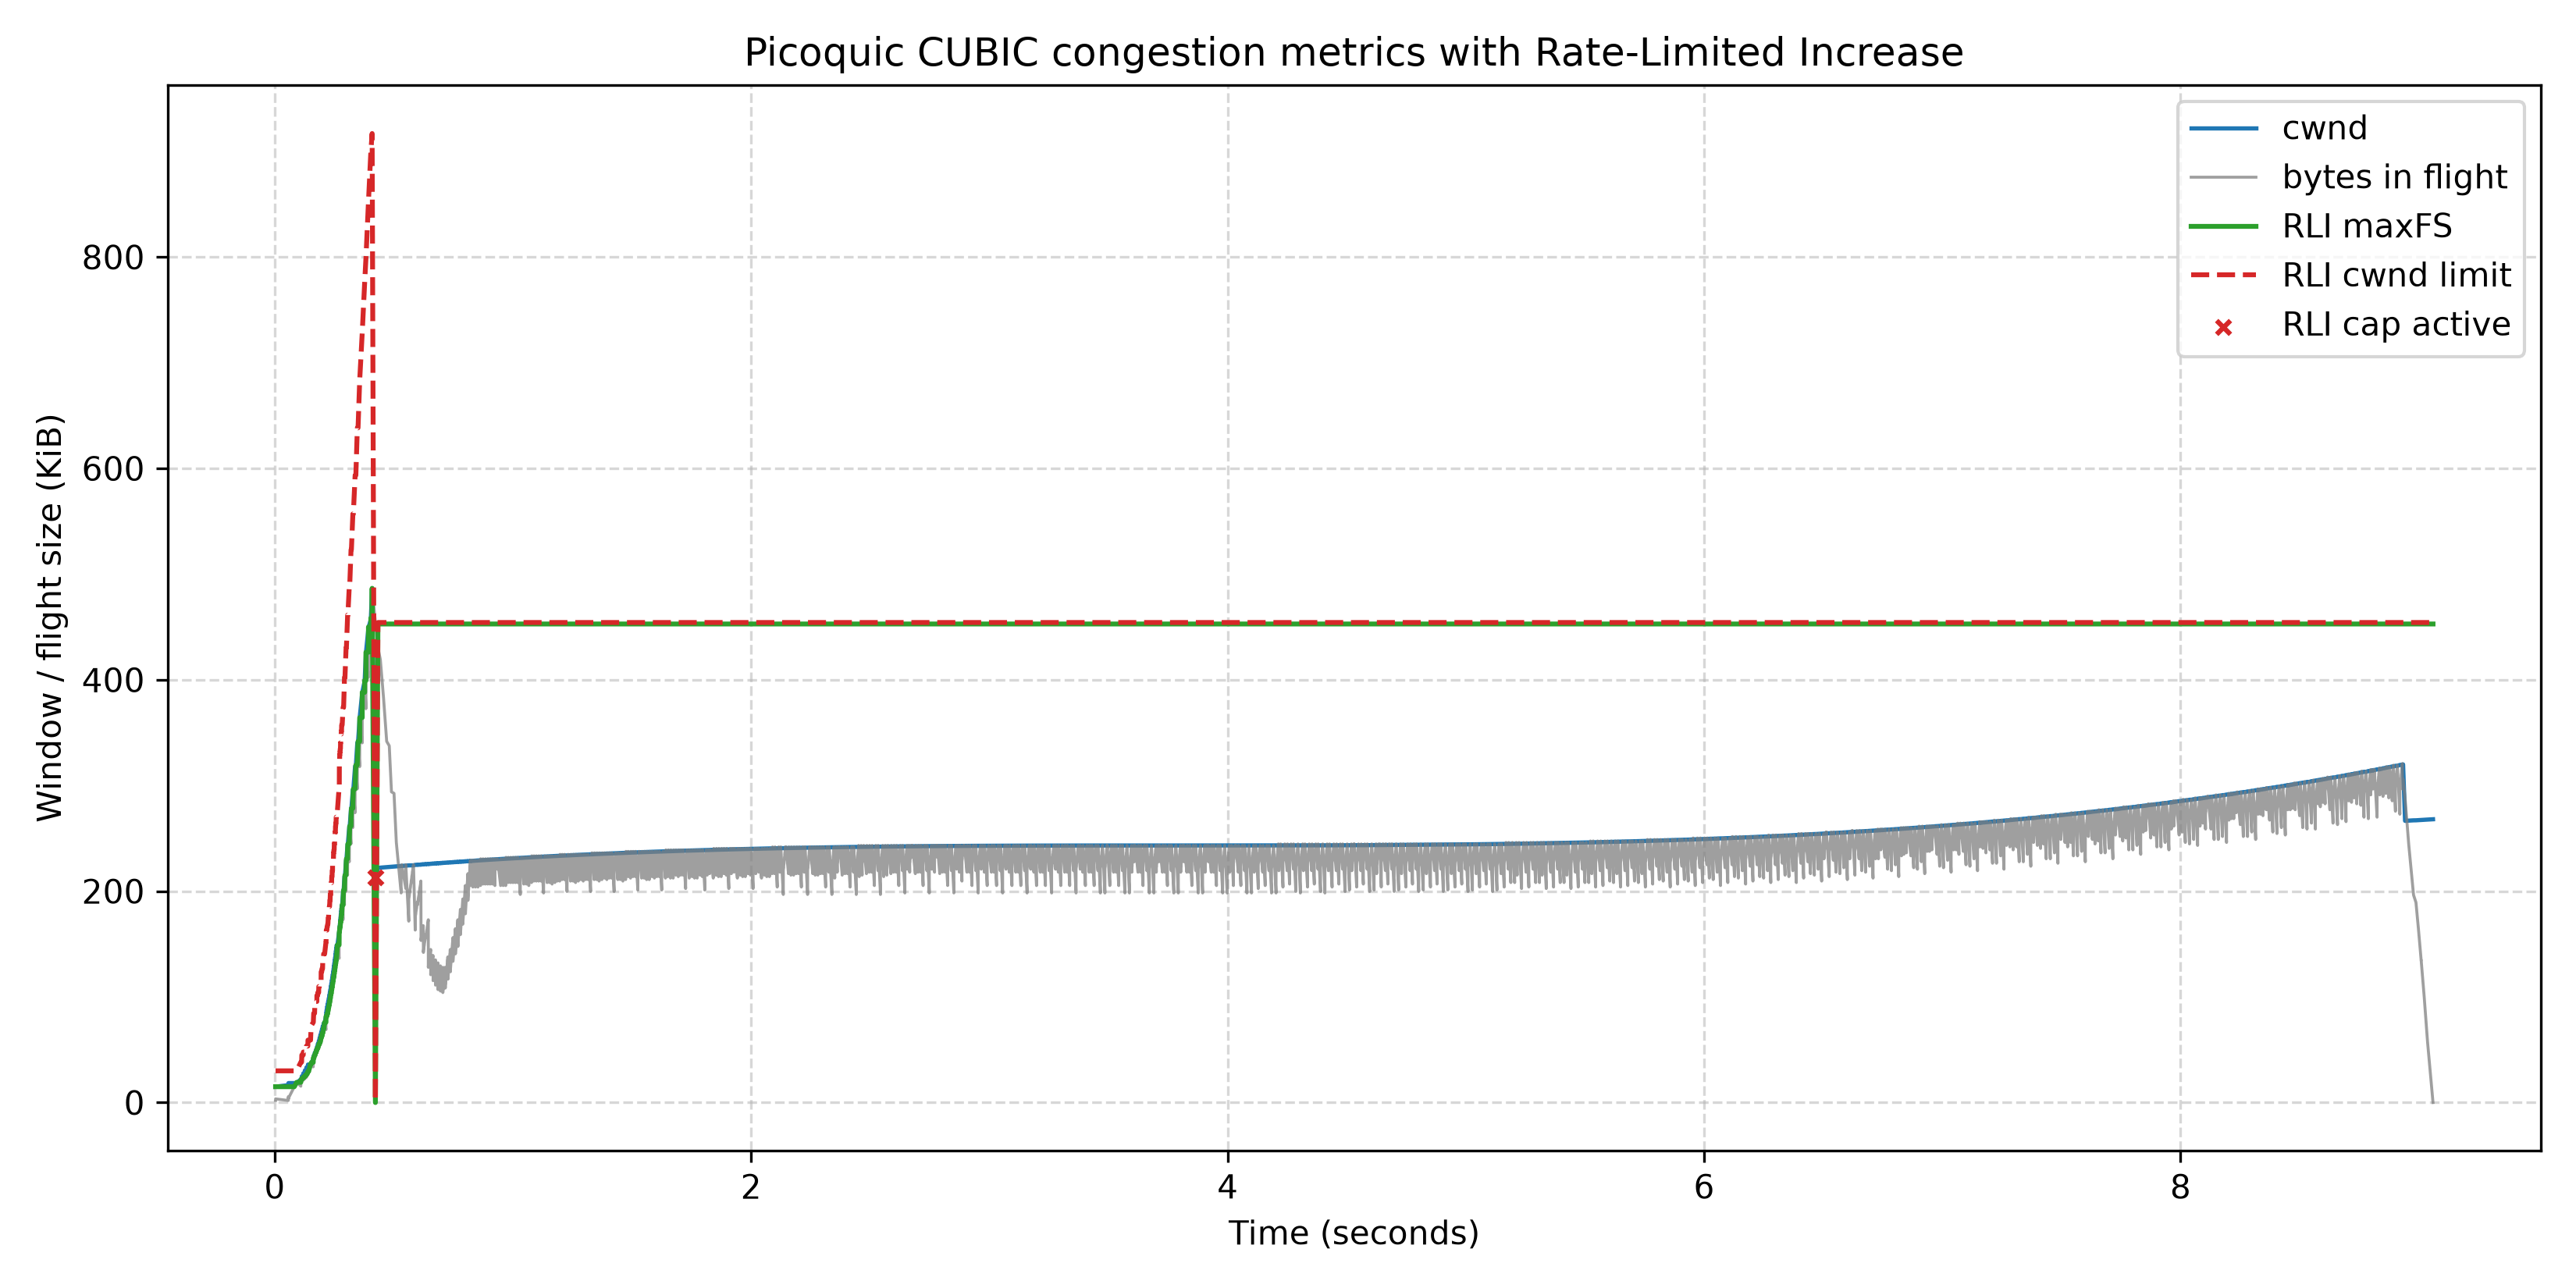
\includegraphics[width=0.92\textwidth]{plots/bulk-rli-1.png}
\caption{Rli: final cwnd 268.04 KiB; time-weighted mean 248.21 KiB; throughput 17.940 Mbit/s.}\end{figure}
These matched traces test a continuously backlogged sender. Normal CUBIC growth and congestion responses dominate; compare measured throughput rather than window height alone.
\clearpage\subsection{Bulk control, repetition 2}
\begin{figure}[H]\centering
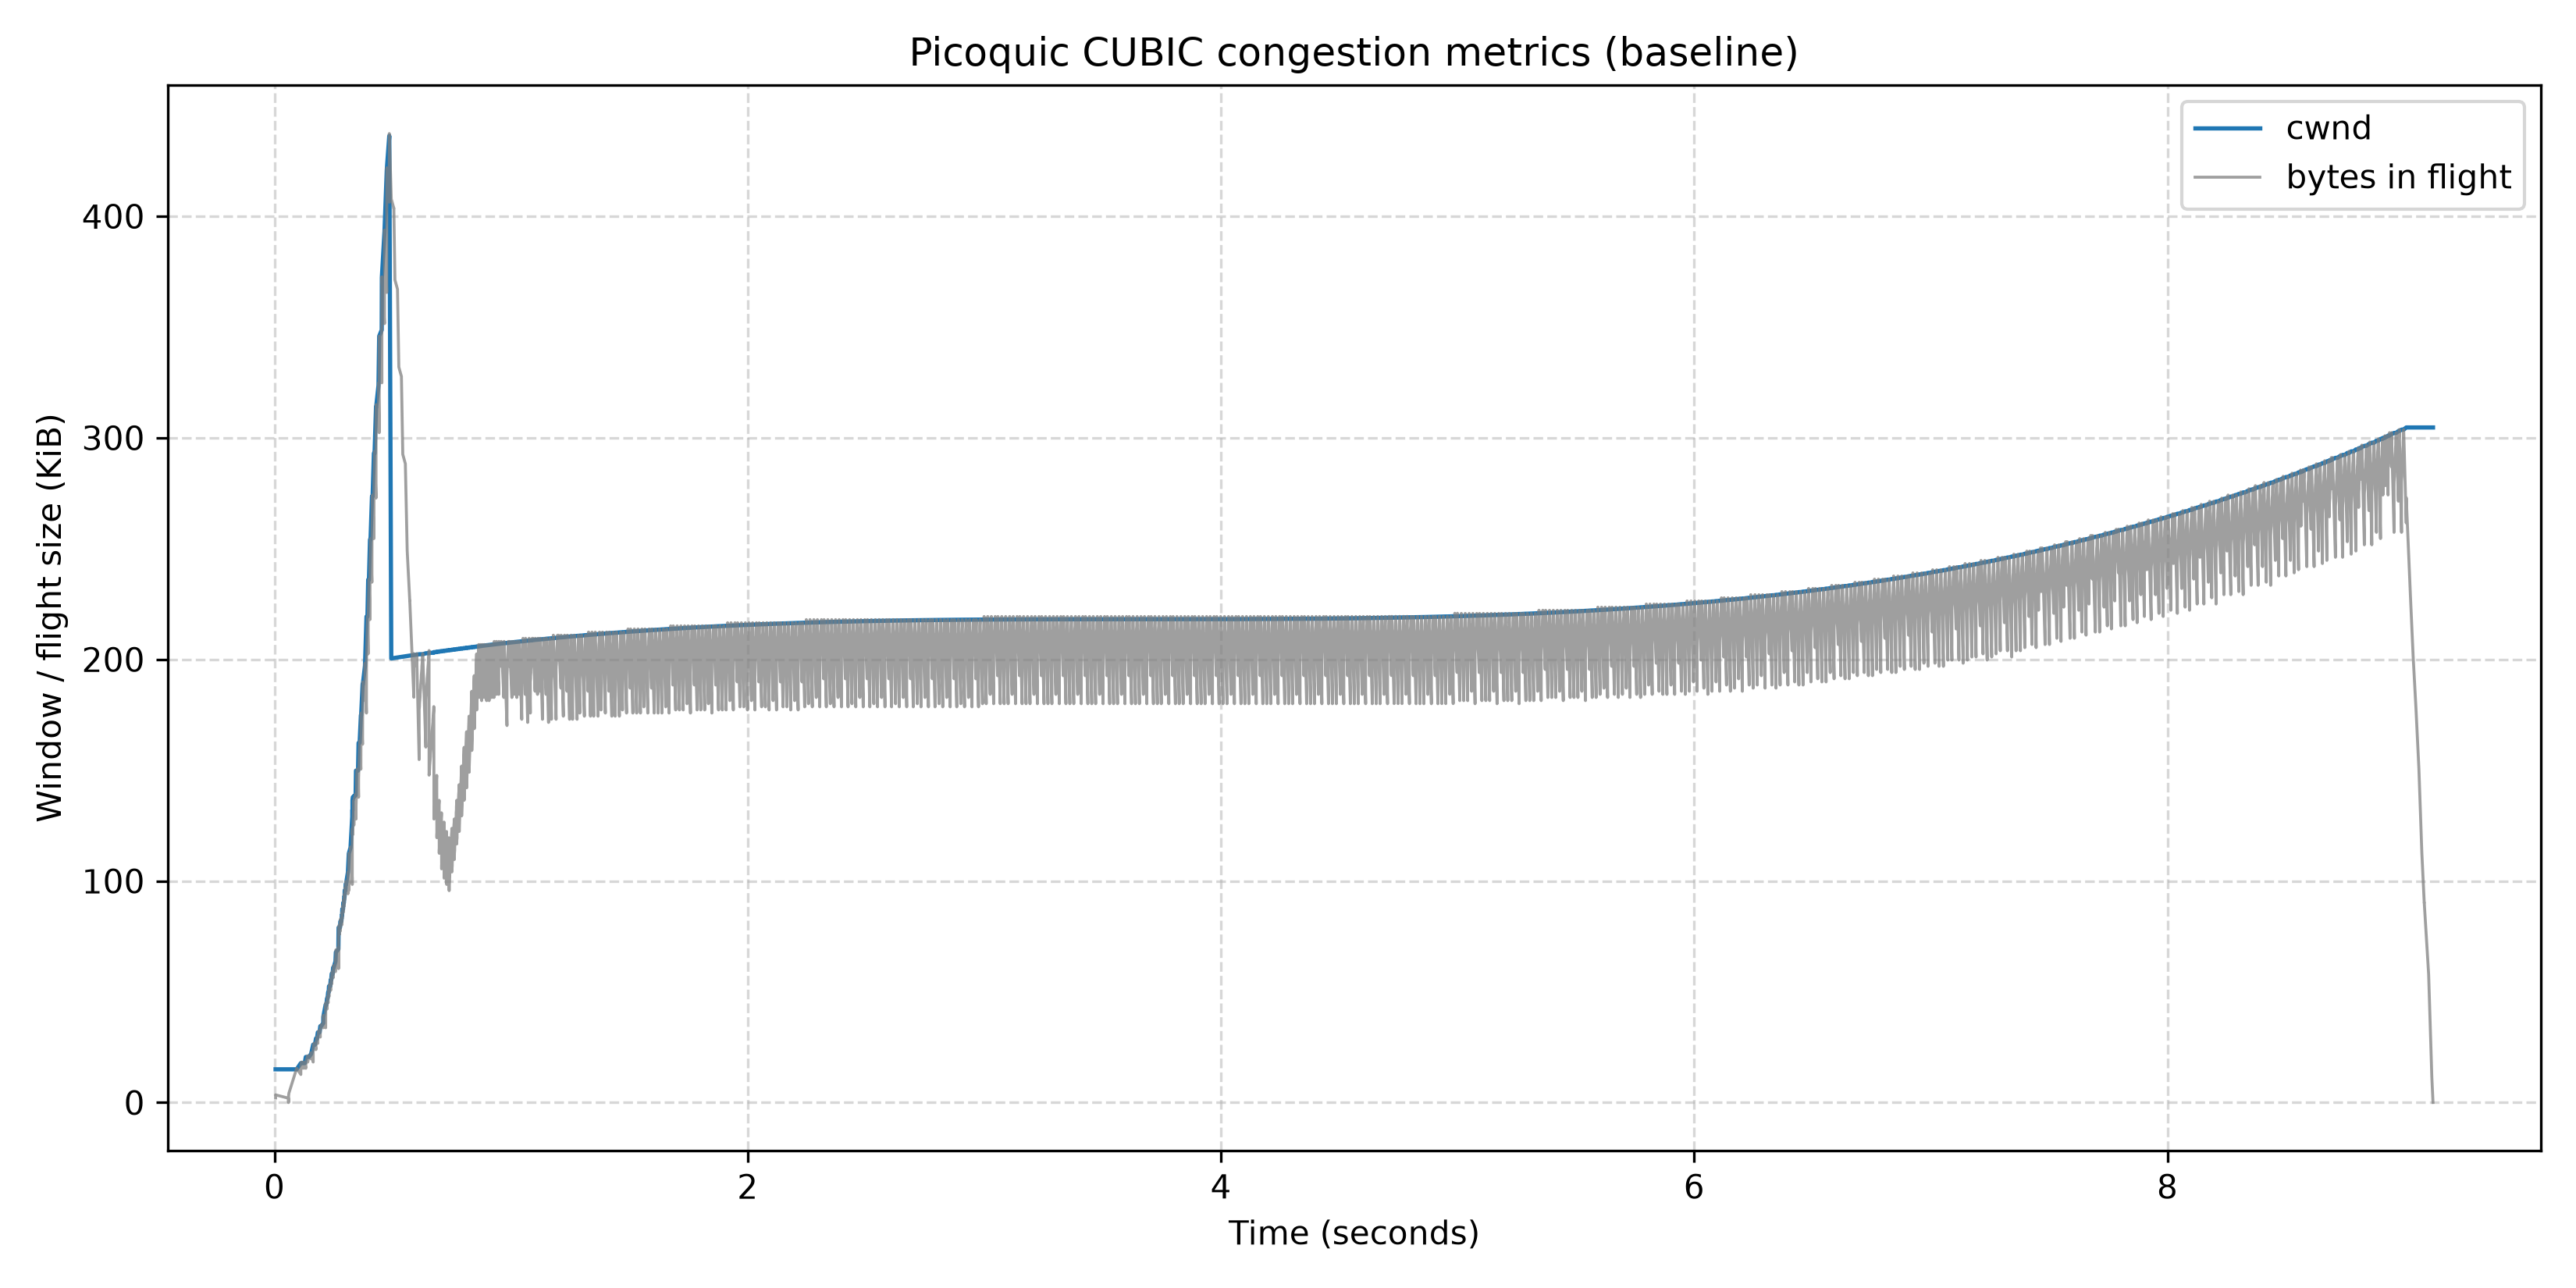
\includegraphics[width=0.92\textwidth]{plots/bulk-baseline-2.png}
\caption{Baseline: final cwnd 304.68 KiB; time-weighted mean 224.90 KiB; throughput 17.823 Mbit/s.}\end{figure}
\begin{figure}[H]\centering
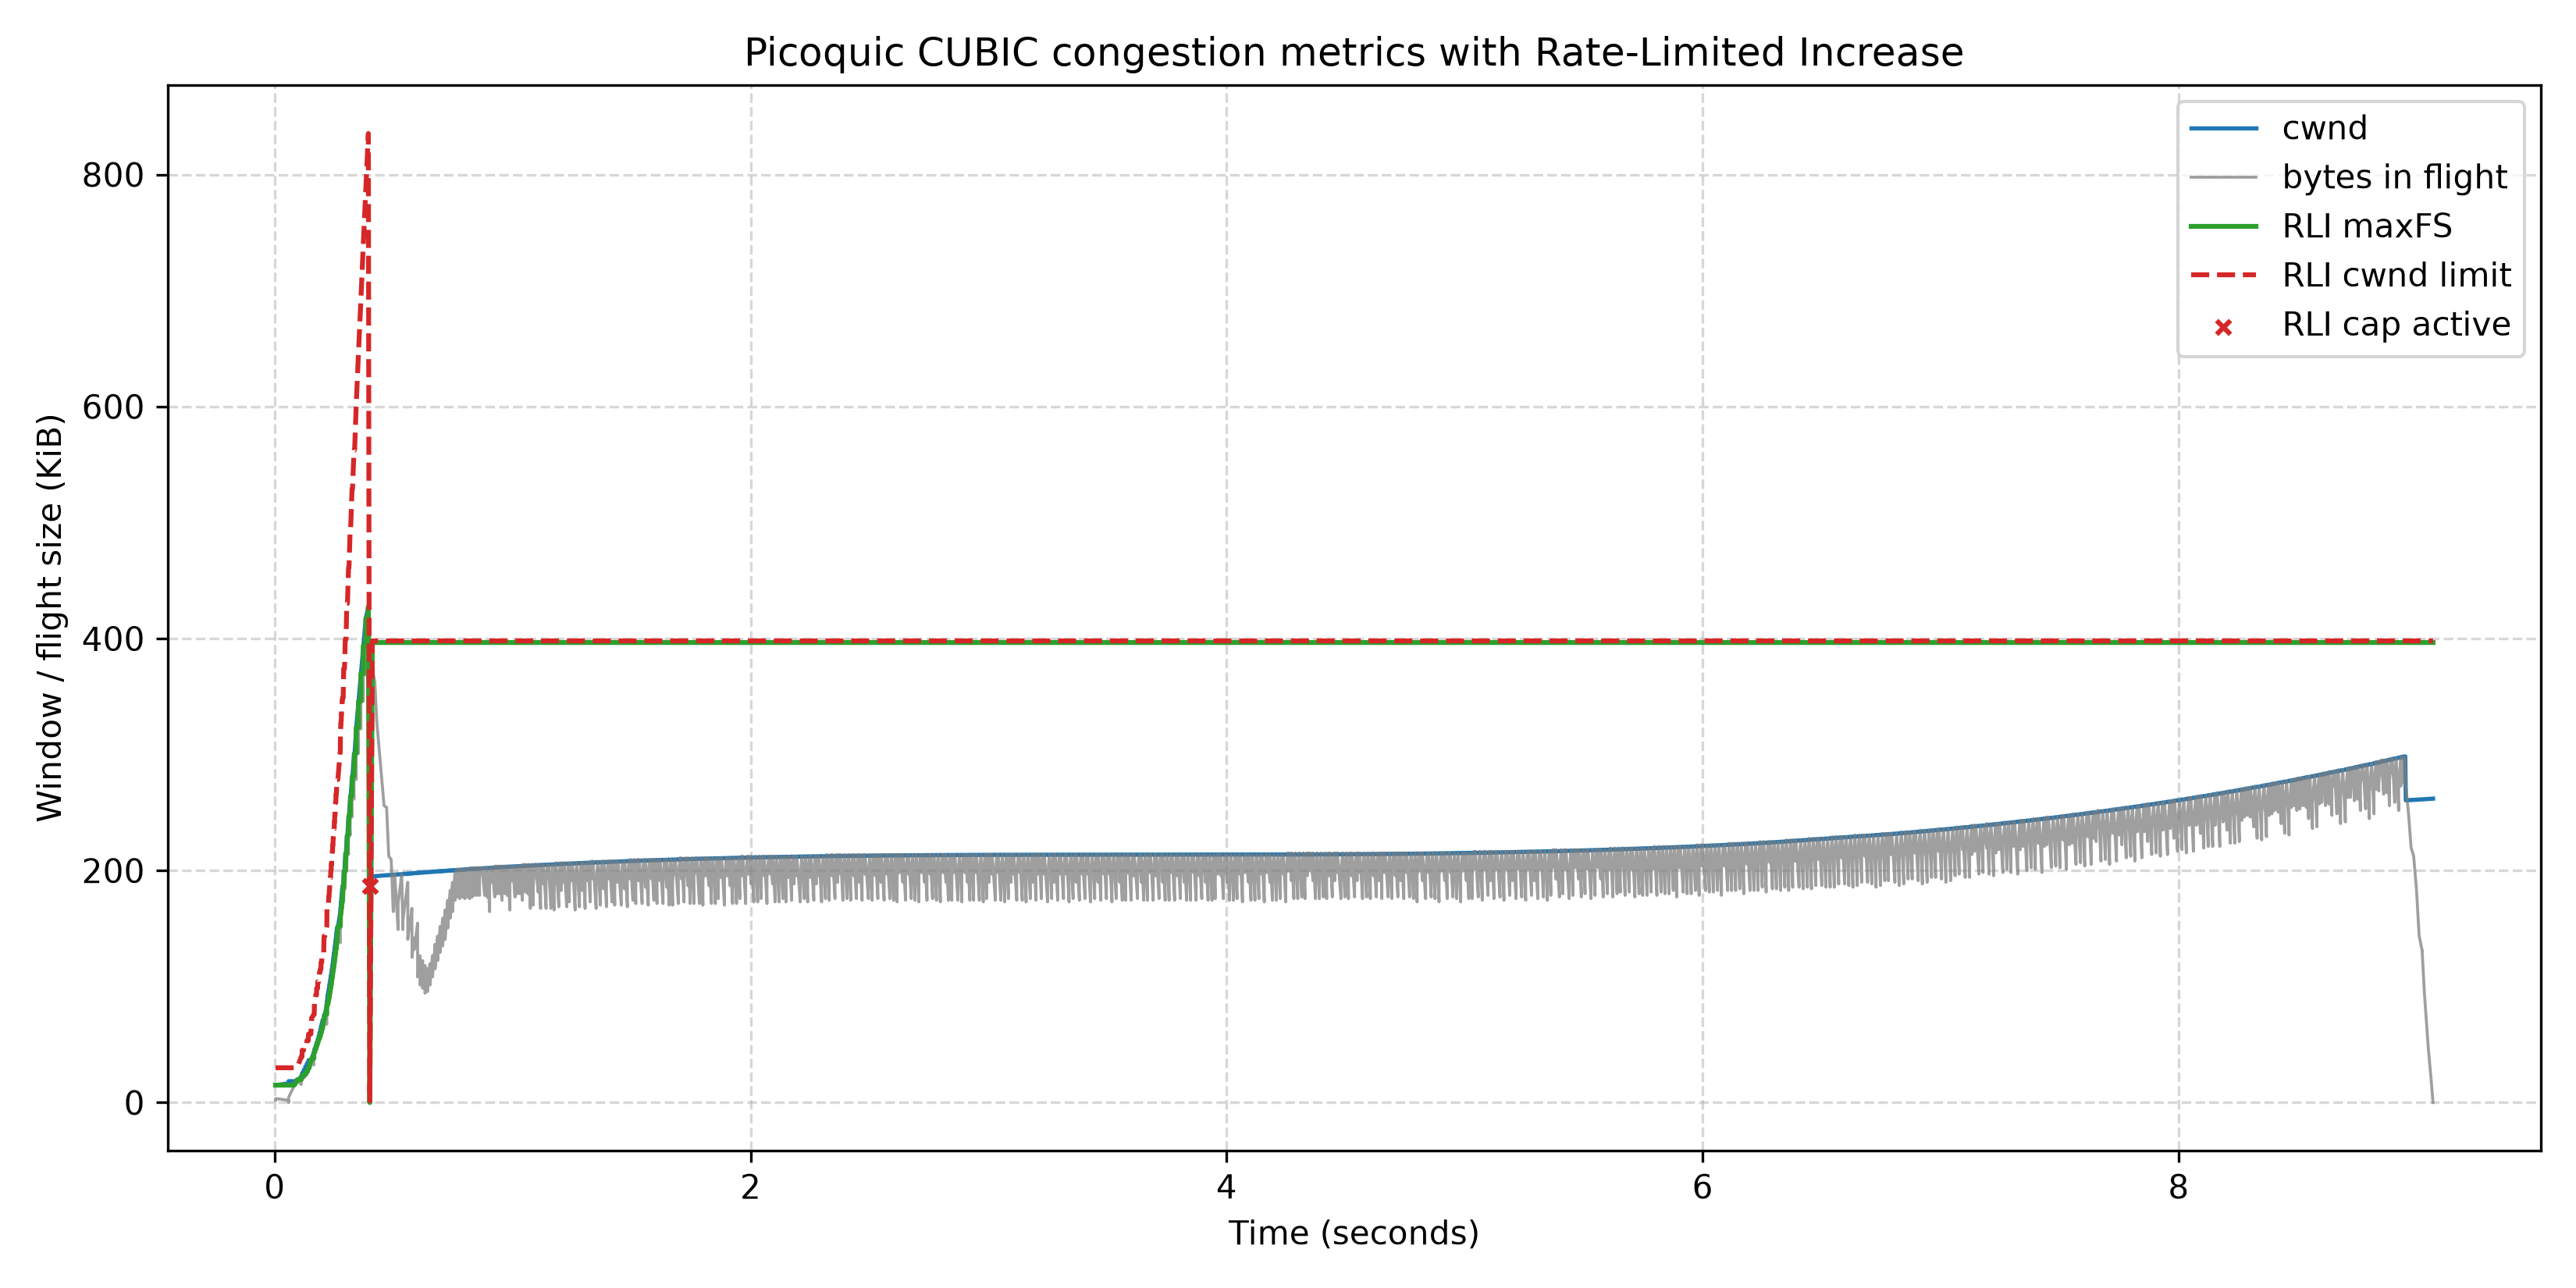
\includegraphics[width=0.92\textwidth]{plots/bulk-rli-2.png}
\caption{Rli: final cwnd 261.98 KiB; time-weighted mean 221.30 KiB; throughput 17.958 Mbit/s.}\end{figure}
These matched traces test a continuously backlogged sender. Normal CUBIC growth and congestion responses dominate; compare measured throughput rather than window height alone.
\clearpage\subsection{Bulk control, repetition 3}
\begin{figure}[H]\centering
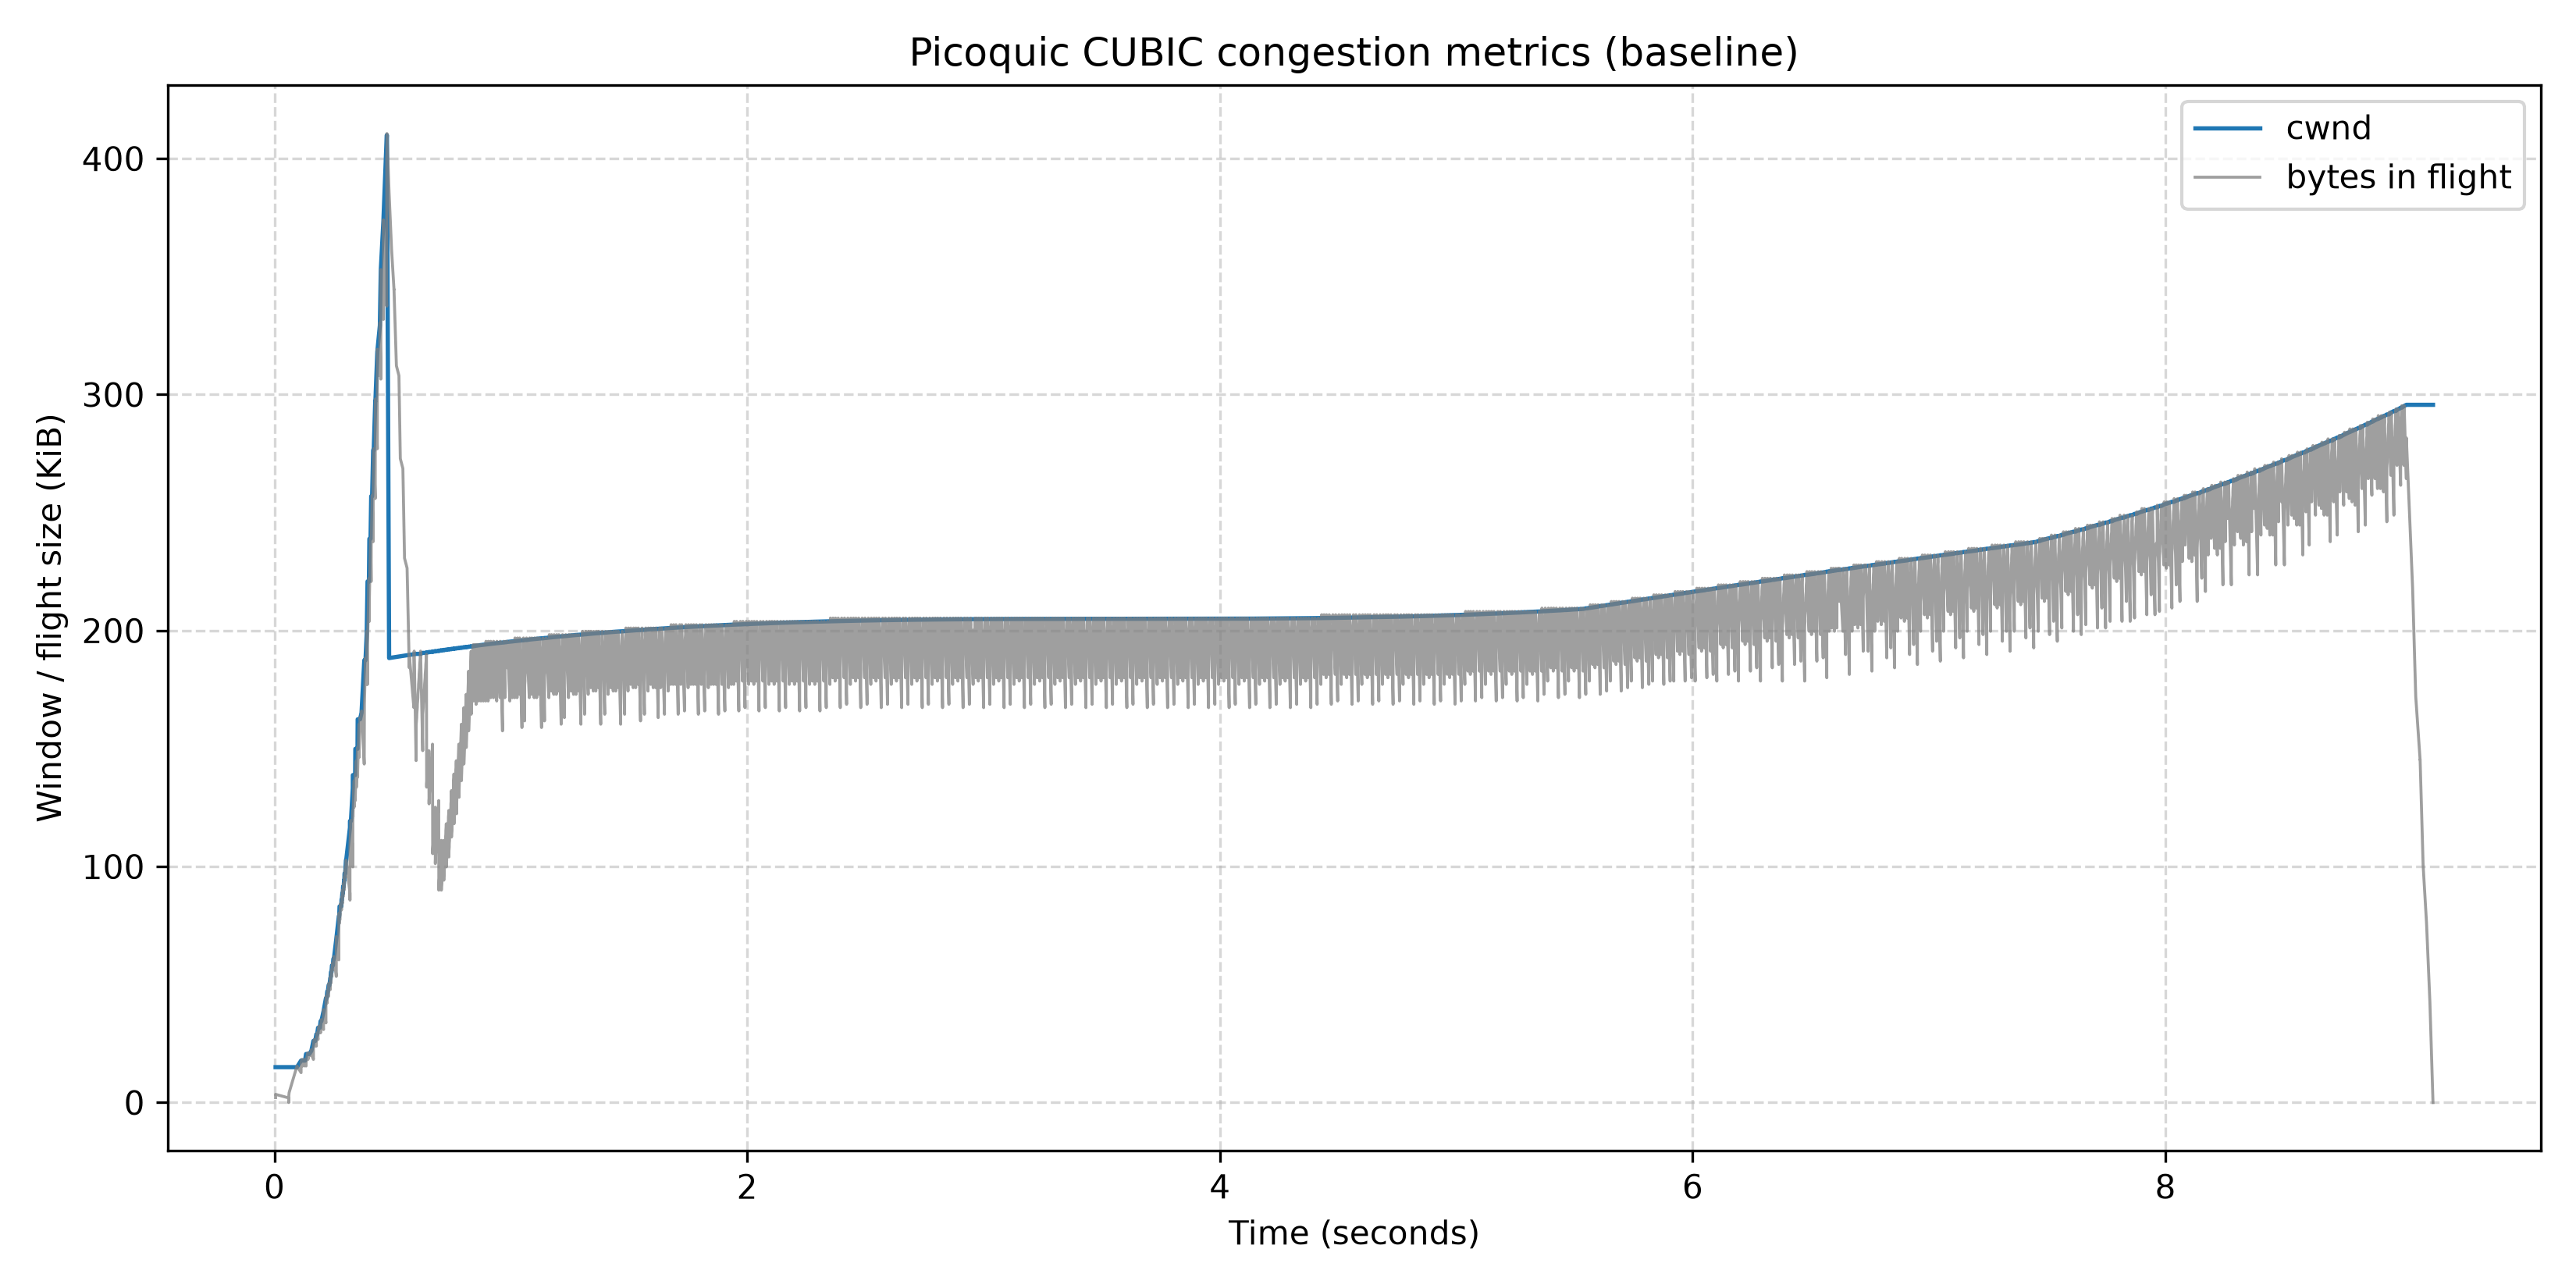
\includegraphics[width=0.92\textwidth]{plots/bulk-baseline-3.png}
\caption{Baseline: final cwnd 295.67 KiB; time-weighted mean 213.74 KiB; throughput 17.640 Mbit/s.}\end{figure}
\begin{figure}[H]\centering
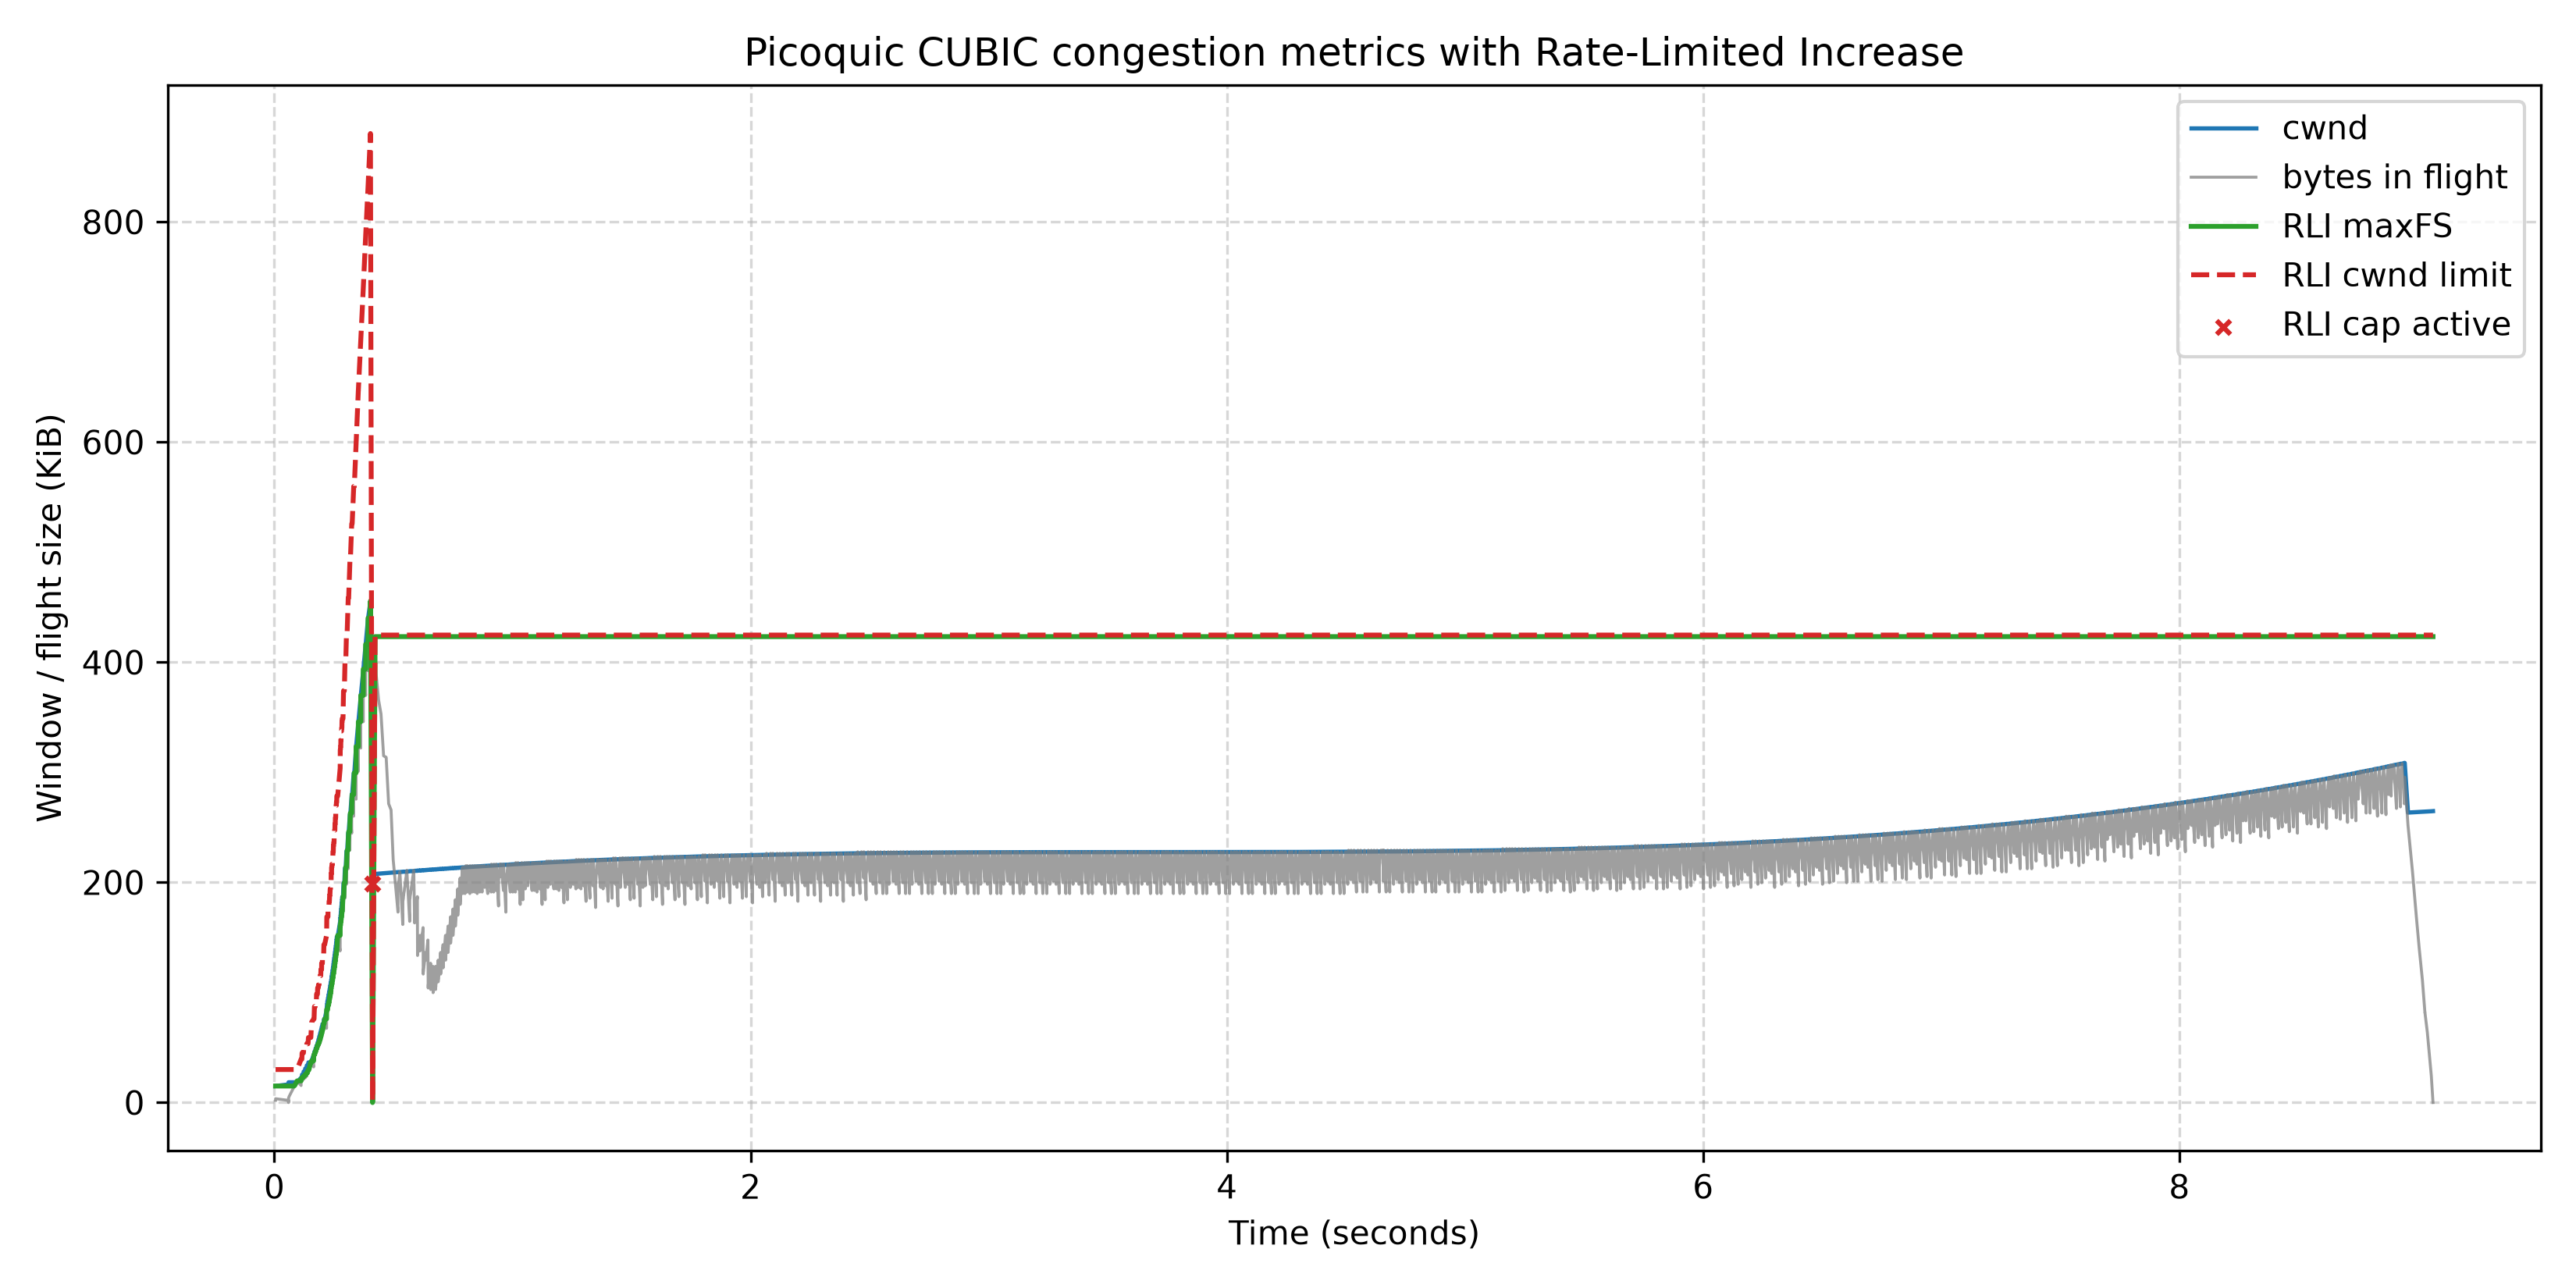
\includegraphics[width=0.92\textwidth]{plots/bulk-rli-3.png}
\caption{Rli: final cwnd 264.75 KiB; time-weighted mean 233.93 KiB; throughput 17.952 Mbit/s.}\end{figure}
These matched traces test a continuously backlogged sender. Normal CUBIC growth and congestion responses dominate; compare measured throughput rather than window height alone.
